\chapter{Vektorkalkulus}
\label{chap:VektorKalk}
I vektorkalkulus er man interessert i deriverte av flervariable funksjoner. I dette kurset er vi mest interessert i funksjoner på $\R^2$ og $\R^3$. 

I og med at $\R^n$ er et vektorrom så skal vi definere en type funksjoner over disse rommene som vi kaller for vektorfelt. Videre skal vi lære å integrere vektorfelt over kurver og flater i $\R^2$ og $\R^3$.

\section{Vektorfelt}\label{sect:vektorfelt}
Generelt sett kaller man en funksjon 
\[\vect{F} \colon \R^n \supseteq U \rightarrow \R^n, \quad \vect{F}=(F_1,\ldots, F_n)^\top\] for et \emph{vektorfelt}. 
For å si det enklere: Se for deg at du knytter en vektor til hvert punkt i rommet. Da har du et felt av vektorer, altså et vektorfelt, over rommet. Et eksempel kan være vannstrøm i en elv. På ethvert punkt i elva kan vi også knytte en vektor, nemlig hastigheten $\vect{v}(x,y,z)$ til vanndråpene. $\vect{v}(x,y,z)$ er da et vektorfelt definert på hele området hvor det er elv. Vektorfelt er altså en type funksjoner, men ofte når vi snakker om funksjoner så tenker vi på $f(x,y,z)$. Følgende terminologi tydeliggjør hva vi mener:
\begin{itemize}
    \item \textit{Skalarfelt}: En funksjon som tilordner en skalar verdi til hvert punkt i rommet. Eksempel: $f(x,y,z)$ over $\R^3$.
    \item \textit{Vektorfelt:} En funksjon som tilordner en vektor til hvert punkt i rommet. Eksempel: $\vect{v}(x,y,z)=(v_1,v_2,v_3)$ over $\R^3$. Merk at komponentene i et vektorefelt er skalare funksjoner, og gjerne varierer over rommet.
\end{itemize}

For å gjøre definisjonen over mer tilgjengelig, tilføyer vi i det følgende mer konkrete definisjoner av vektorfelt for $\R^2$ og $\R^3$.

\begin{defn}{Vektorfelt i 2D og 3D}
Et \emph{vektorfelt} i to eller tre dimensjoner er en funksjon som til hvert punkt $(x, y)$ eller $(x, y, z)$ tildeler en vektor:
\[
\vect{F}(x, y) = P(x, y)\,\vect{i} + Q(x, y)\,\vect{j}, \quad
\vect{G}(x, y, z) = P(x, y, z)\,\vect{i} + Q(x, y, z)\,\vect{j} + R(x, y, z)\,\vect{k}
\]
Her er altså $P$, $Q$ og $R$ komponentene til vektoren $\vect{F}$. I stedet for å bruke $P$, $Q$ og $R$ for å angi komponentene, kunne vi brukt $F_1,F_2$ og $F_3$. Noen av oss kommer til å bruke dette i forelesning.
\end{defn}

\begin{eks}{Å skissere vektorfelt}
Skissér følgende vektorfelt:
\begin{itemize}
  \item[a)] $\vect{F}(x, y) = 2y\,\vect{i} + x\,\vect{j}$
  \item[b)] $\vect{F}(x, y, z) = \sin(\pi x)\cos(\pi y) \cos(\pi z)\,\vect{i} - \cos(\pi x)\sin(\pi y)\cos(\pi z)\,\vect{j} + \cos(\pi x) \cos(\pi y) \sin(\pi z)\,\vect{k}$
\end{itemize}
Den enkleste måten å skissere vektorfelt på er å bruke Python. I noen tilfeller, slik som i oppgave b, er det også den mest fornuftige tilnærmingen. Sjekk ut JuPyter-notatet vårt om vektorfelt! 
\end{eks}
For 3D-vektorfelt er det ofte best å bruke et dataverktøy som Python for å tegne dem. 
\begin{minipage}{\columnwidth}
\begin{oppsum}{\textbf{Nyttige Python kommandoer}}
\begin{minipage}{.9\columnwidth}
\begin{lst}{}
import numpy as np

import matplotlib.pyplot as plt

np.meshgrid

plt.quiver
\end{lst}
\end{minipage}
\end{oppsum}
\end{minipage}
La oss nå introdusere $\nabla$-operatoren (uttale: nabla) og vise hvordan denne lager et vektorfelt $\nabla f$ av en funksjon $f$.

\begin{defn}{Nabla-operatoren ($\nabla$)} For $\R^n$ er \emph{Nabla operator} definert som
\[\nabla := \sum_{i=1}^n \frac{\partial}{\partial x_i}\, \vect{e}_i , \quad \text{ hvor } \vect{e}_i = (0,\ldots, 1, 0\ldots, 0)^\top\]
I to-og tredimensjonale rom gir dette de konkretere formlene
\begin{align*}
\nabla &= \frac{\partial}{\partial x}\, \vect{i} + \frac{\partial}{\partial y}\, \vect{j} \qquad \qquad  \text{ i 2D}\\
\nabla &= \frac{\partial}{\partial x}\, \vect{i} + \frac{\partial}{\partial y}\, \vect{j} + \frac{\partial}{\partial z}\, \vect{k} \quad \text{ i 3D}
\end{align*}
\label{defn:nabla}
\end{defn}
Vi kan se på $\nabla$ som en vektor.  Om vi nå anvender $\nabla$-operatoren direkte på en funksjon $f$, så får vi et vektorfelt:
\[
\nabla f = \frac{\partial f}{\partial x}\, \vect{i} + \frac{\partial f}{\partial y}\, \vect{j} + \frac{\partial f}{\partial z}\, \vect{k}
\]
Vi ser altså at $\nabla f$ gir oss de partielle deriverte av \(f(x,y,z)\) i hvert punkt $(x,y,z)$. Dette vektorfeltet kan også kalles \(\text{grad } f (x,y,z)\), og blir viktig i den videre diskusjonen i dette kapitlet.

\begin{defn}{Gradientvektorfelt}
Gitt en funksjon  $\vect{F}\colon \R^n \supseteq U \rightarrow \R$ så definerer vi
\[
\text{grad } f (x_1,\ldots, x_n) :=\nabla f= \sum_{i=1}^n \frac{\partial f}{\partial x_i}\vect{e}_i
\]
Dette vektorfeltet kalles \emph{gradient-vektorfeltet}, eller bare \textit{gradienten}, til $f$.
\end{defn}

\begin{eks}{Gradienter}
Finn gradientvektorfeltet for følgende funksjoner:
\begin{itemize}
  \item[a)] $f(x, y) = x^2\cos(5y) \quad  \Rightarrow \nabla f (x,y)= (2x\cos(5y), -5x^2\sin(5y) )^\top$
  \item[b)] $f(x, y, z) = ze^{-xy} \qquad  \Rightarrow \nabla f(x,y,z) = ( -yze^{-xy}, -xze^{-xy}, e^{-xy} )^\top$
\end{itemize}
\end{eks}
\begin{eks}{Gradienter og nivåkurver}
Skisser gradientvektorfeltet og nivåkurvene til $f(x, y) = x^2 + y^2$. Nivåkurver er gitt av:
\[
f(x, y) = k \Rightarrow x^2 + y^2 = k
\]
Dette er sirkler med radius $\sqrt{k}$.
Gradienten er:
\[
\nabla f(x, y) = 2x\,\vect{i} + 2y\,\vect{j}
\]
Vektorene er ortogonale på nivåkurvene og peker i retning av raskest endring.
\end{eks}
\begin{oppsum}{Fakta om gradienter}
For en reellverdig funksjon $f$ gjelder for grad $f$ at det
\begin{itemize}
\item peker i hver punkt i retning hvor $f$ har størst endring.
\item står ortogonalt på nivåkurvene til $f$.
\end{itemize}
\end{oppsum}
\begin{defn}{Konservative vektorfelt}
Et vektorfelt $\vect{F}$ er \emph{konservativt} hvis det finnes en funksjon $f$ slik at:
\[
\vect{F} = \nabla f
\]
Da er $f$ en \emph{potensialfunksjon} for $\vect{F}$. Man sier også kortere at $f$ er en potensial for $\vect{F}$
\end{defn}

\begin{eks}{}
\begin{itemize}
    \item $\vect{F} = y\, \vect{i} + x\, \vect{j}$ er konservativt, med potensialfunksjon $f(x, y) = xy$
    \item $\vect{F} = -y\, \vect{i} + x\, \vect{j}$ er ikke konservativt. Vi skal senere begrunne hvorfor det ikke er konservativt.
\end{itemize}
\end{eks}

Teorien for ordinære differensiallikninger (ODE-er) kan betraktes geometrisk som et svar på spørsmålet: Gitt et vektorfelt i \( \mathbb{R}^n \) og et punkt \( p_0 \) i \( \mathbb{R}^n \), kan man finne en kurve \( \gamma \) gjennom \( p_0 \) slik at tangentvektoren i hvert punkt \( p \) på \( \gamma \) samsvarer med verdien til vektorfeltet i \( p \)?

La oss forsøke å visualisere denne ideen for $n=2$. Et vektorfelt i \( \mathbb{R}^2 \) er gitt ved en avbildning  
\[
\vect{v} : \mathbb{R}^2 \rightarrow \mathbb{R}^2, \vect{v}(x,y)= P(x,y)\vect{i} + Q(x,y)\vect{j}
\]
Vi leter nå etter en kurve  
\[
\vect{r}(t) = x (t) \vect{i} + y(t) \vect{j},
\]  
som oppfyller betingelsene  
\begin{align}\label{tangent:curve}
\frac{d\vect{r}}{dt}(t) = \vect{v}(\vect{r}(t))= P(\vect{r}(t)) \vect{i} + Q(\vect{r}(t))\vect{j}
\end{align}  
samt initialbetingelsene (som sier at kurven går gjennom et gitt punkt \( p_0 =(x_0,y_0)\) for en (initial) verdi \( t_0 \) av parameteren \( t \). Vi ser at den geometriske krav om tangenten til kurven er det gitte vektorfeltet oversettes til den analytiske formuleringen i ligning \eqref{tangent:curve}, som ganske enkelt er et system av ordinære differensiallikninger (ODE-er) av første orden.

\begin{rem}{}
Dersom vektorfeltet forsvinner (er null) i et punkt \( P \), er løsningen av \eqref{tangent:curve} gjennom \( P \) konstant, slik at hele kurven kollapser til et punkt. Vi sier da at \( P \) er en likevektstilstand for systemet.
\end{rem}

\begin{eks}{}
Se på vektorfelt
$
\vect{F}(x,y)= y\vect{i} - \sin (x) \vect{j}
$ (JuPyter notat for visualisering).
La oss nå vilkårlig velge et startpunkt \(\vect{r}_0 = -9 \vect{i}+  2\vect{j} \).  

Vi ønsker å finne en kurve som, idet den passerer gjennom dette punktet, alltid er tangent til den lokale verdien av $\vect{F}$. Med andre ord ønsker vi å løse følgende ikke-lineære system av ordinære differensiallikninger:
\begin{align*}
\frac{dx}{dt} &= y(t), \quad x(0)=-9 \\
\frac{dy}{dt} &= -\sin (x(t)), \quad y(0)=2.
\end{align*}
Numerisk løsning til dette, samt visualisering, ligger i JuPyter notatet (Sjekk JuPyter!). Se figur~\ref{fig:flow}.
\end{eks}
\begin{figure}
    \centering
    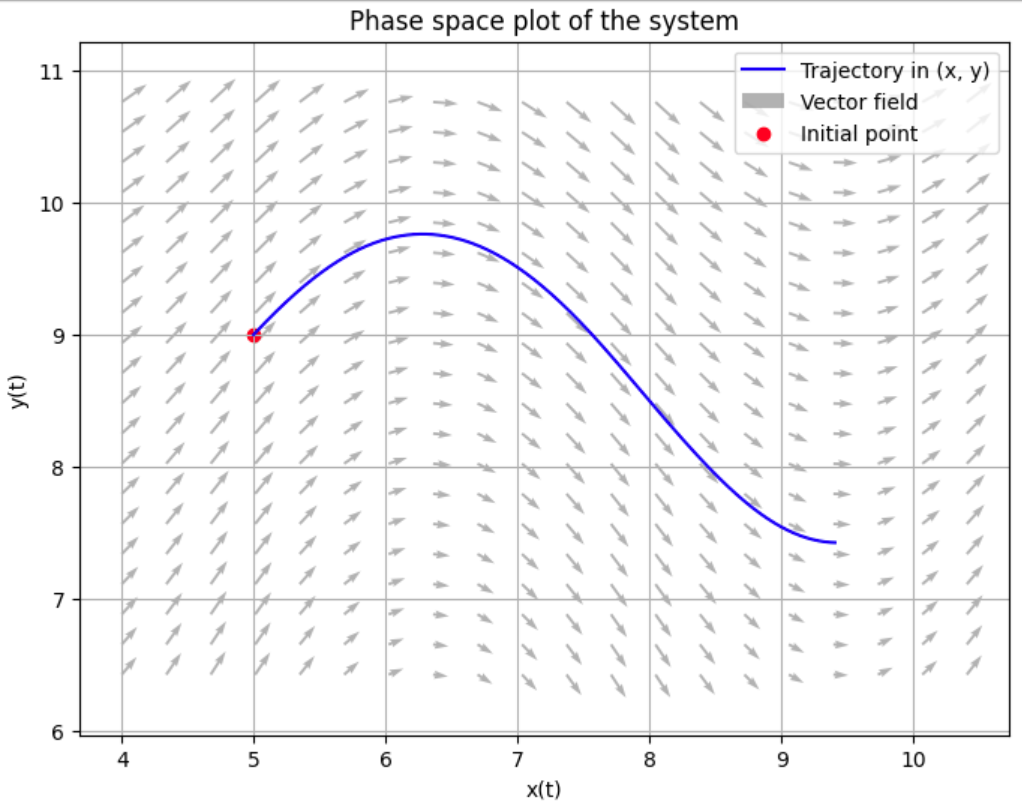
\includegraphics[width=0.8\linewidth]{Fig/ParticleFlow.png}
    \caption{Figuren viser en partikkel som følger vektorfeltet $\vect{F}(x,y)= y\vect{i} - \sin (x) \vect{j},$ med startposisjon $\vect{r}_0=5\vect{i}+9\vect{j}$.}
    \label{fig:flow}
\end{figure}

%
%
%
\section{Divergens og rotasjon (curl)}\label{div_curl}

I dette kapitlet introduserer vi begrepene \textbf{rotasjon} (curl) og \textbf{divergens}. 

\begin{defn}{Divergens}
For et vektorfelt $\vect{F}\colon \R^n\rightarrow \R^n , \vect{F}=(F_1,\ldots, F_n)$ er \emph{divergensen} til $\vect{F}$ definert som 
\[\text{div }\vect{F} := \nabla\cdot \vect{F}=\sum_{i=1}^n \frac{\partial F_i}{\partial x_i},\]
hvor $\nabla=(\frac{\partial}{\partial x_1},\frac{\partial}{\partial x_2},..., \frac{\partial}{\partial x_n})$ som før, se Definisjon~\ref{defn:nabla}.
\end{defn}
Dersom vi spesialiserer definisjonen til to dimensjoner ser vi at dette gir 
\begin{align*}
\vect{F} = P\vect{i} + Q\vect{j}\quad\Rightarrow\quad\nabla\cdot\vect{F} = \frac{\partial P}{\partial x} + \frac{\partial Q}{\partial y},
\end{align*}
På tilsvarende vis får vi i tre dimensjoner at
\begin{align*}
\vect{F} = P\vect{i} + Q\vect{j} + R\vect{k}\quad\Rightarrow\quad\nabla\cdot\vect{F} = \frac{\partial P}{\partial x} + \frac{\partial Q}{\partial y} + \frac{\partial R}{\partial z} .
\end{align*}


\begin{eks}{}
Gitt $\vect{F}(x,y,z) = x^2y \vect{i} + xyz \vect{j} - x^2y^2 \vect{k}$.
\[
\text{div } \vect{F} = 2xy + xz
\]
\end{eks}{}
\paragraph{Fysisk tolkning av divergens:} Dersom vi tenker oss at $\vect{F}$ er hastighetsfeltet til en gass (eller en væske), representerer $\text{div }\vect{F}$ ekspansjonshastigheten per volumenhet i strømmen av gassen (eller væsken). 
Dersom $\text{div } \vect{F} < 0$, betyr det at gassen (eller væsken) komprimeres.

For et vektorfelt $\vect{F}(x, y) = F_1 \vect{i} + F_2 \vect{j}$ i planet er divergensen gitt ved
\[
\nabla \cdot \vect{F} = \frac{\partial F_1}{\partial x} + \frac{\partial F_2}{\partial y},
\]
og dette uttrykket måler arealekspansjonshastigheten.
Denne tolkningen kan illustreres grafisk på følgende måte:

\begin{figure}[ht!]
    \centering
    % Første figur
    \begin{subfigure}[b]{0.45\textwidth}
        \centering
        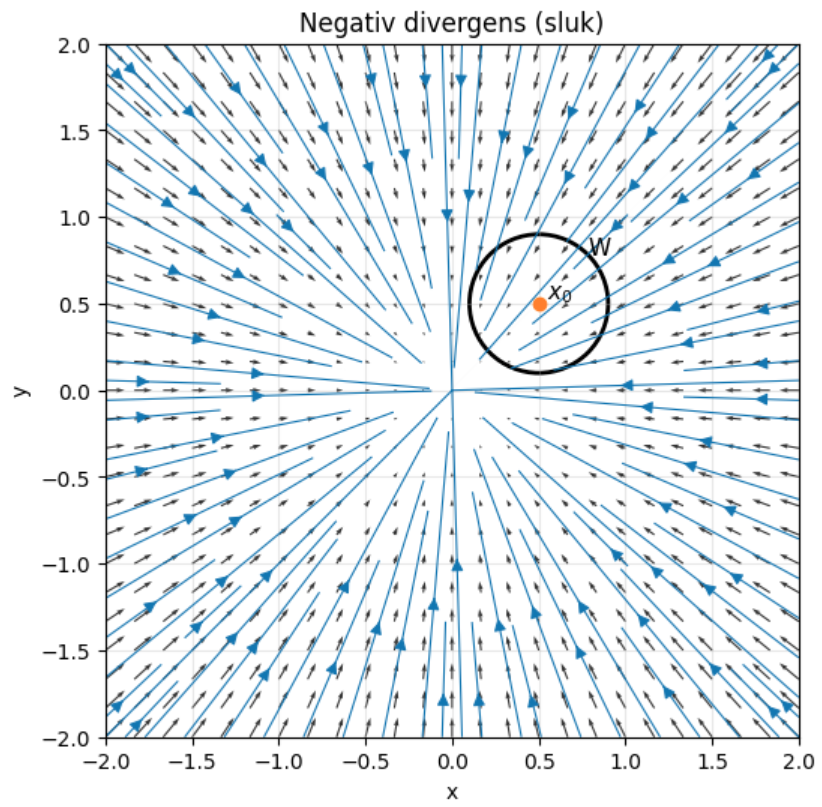
\includegraphics[width=\textwidth]{Fig/fig_sink.png}
        \caption{Bildet viser strømlinjer og vektorfelt for $\vect{F}=-x\vect{i}-y\vect{j}$ i planet.}
        \label{fig_sink}
    \end{subfigure}
    \hfill
    % Andre figur
    \begin{subfigure}[b]{0.45\textwidth}
        \centering
        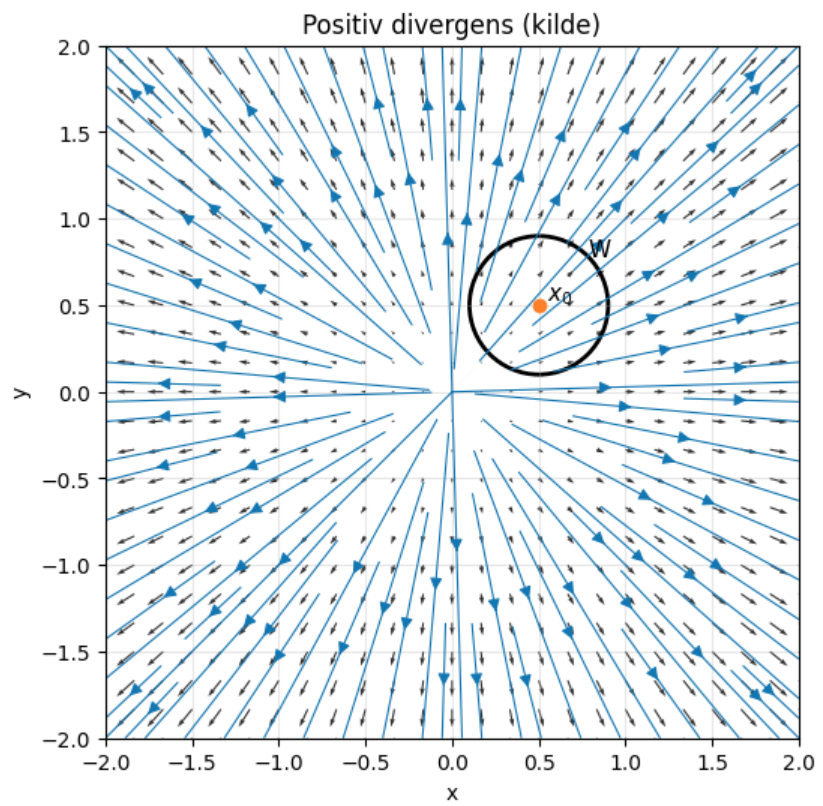
\includegraphics[width=\textwidth]{Fig/fig_source.png}
        \caption{Bildet viser strømlinjer og vektorfelt for $\vect{F}=x\vect{i}+y\vect{j}$ i planet.}
        \label{fig:source}
    \end{subfigure}
    \caption{To eksempler på vektorfelt med divergens ulik null.}
    \label{fig:tofigurer}
\end{figure}


Velg et lite område $W$ rundt et punkt $x_0$. For hvert punkt $x$ i $W$, la $x(t)$ være strømlinjen til $\vect{F}$ som går ut fra $x$. Mengden av punkter $x(t)$ beskriver hvordan området $W$ flyter etter tid $t$. 
La området etter tid $t$ være $W(t)$, og la $V(t)$ være volumet (eller arealet i to dimensjoner) til $W(t)$. Da er den relative veksthastigheten til volumet gitt av divergensen. Mer presist:
\[
\left. \frac{1}{V(0)} \frac{dV(t)}{dt} \right|_{t=0} \approx \text{div }\vect{F}(x_0),
\]
og denne tilnærmelsen blir mer nøyaktig jo mindre området $W$ er, altså når $W \to x_0$.


Vi kommer nå til rotasjon.\footnote{På norsk kan man også bruke betegnelsen 'rot' for rotasjon, men siden det ikke er i bruk i internasjonal litteratur bruker vi heller curl som er engelsk for rotasjon.}

\begin{defn}{Rotasjon (på engelsk curl)}
Gitt vektorfeltet
\[
\vect{F} = P\, \vect{i} + Q\, \vect{j} + R\, \vect{k}
\]
defineres \emph{rotasjonen} (engelsk: \emph{curl}) som:
\[
\text{curl } \vect{F} :=\nabla\times\vect{F}=
\left( \frac{\partial R}{\partial y} - \frac{\partial Q}{\partial z} \right)\vect{i}
+ \left( \frac{\partial P}{\partial z} - \frac{\partial R}{\partial x} \right)\vect{j}
+ \left( \frac{\partial Q}{\partial x} - \frac{\partial P}{\partial y} \right)\vect{k}
\]
\label{defn:curl}
\end{defn}

\begin{rem}{}
 curl er {\large kun} definert i tre dimensjoner.
\end{rem} 

\paragraph{Beregning av rotasjon ved hjelp av determinant}
Når vi skal beregne curlen kan det være lurt å benytte en determinant for utregningen, slik man gjerne gjør for kryssprodukt:
\[
\text{curl } \vect{F} = \nabla \times \vect{F} =
\begin{vmatrix}
\vect{i} & \vect{j} & \vect{k} \\
\frac{\partial}{\partial x} & \frac{\partial}{\partial y} & \frac{\partial}{\partial z} \\
P & Q & R.
\end{vmatrix}
\]
Dette er ekvivalent med definisjonen~\ref{defn:curl} over.


\paragraph{Fysisk tolkning av rotasjon} Hvis $\vect{F}$ er hastighetsfeltet til en væskestrøm så representerer $\text{curl } \vect{F}$ partiklenes tendens til å (i ethvert punkt) rotere rundt en akse i retningen til $\text{curl } \vect{F}$. Spesielt betyr $\text{curl } \vect{F} = 0$ i et punkt $P$ at væsken er fri for stive rotasjoner i $P$; det vil si at det ikke finnes noen virvler i punktet. 

En annen begrunnelse for denne tolkningen kommer fra Stokes' teorem \Cref{thm:stokes} vi skal se senere på. Likevel kan vi uformelt si at $\text{curl } \vect{F} = 0$ betyr at hvis et lite stivt skovlhjul plasseres i væsken, vil det følge med strømmen, men ikke rotere rundt sin egen akse. Et slikt vektorfelt med $\text{curl } \vect{F} = 0$ kalles \emph{irrotasjonelt}.

Eksperimenter vist at væske som renner ut av et badekar vanligvis er irrotasjonell — bortsett fra helt i sentrum — selv om væsken “roterer” rundt sluket. 


\begin{eks}{}\label{ex:irrot}
Strømlinjene til vektorfeltet \[\vect{F}(x,y,z) = \frac{y\vect{i}-x\vect{j}}{x^2+y^2}\]
er sirkler rundt origo, se figur~\Cref{fig:rotasjonsFritt} og~\Cref{fig:VF-irrot}. Feltet er definert på $\R^3 \setminus \{\vect{0}\}$ og er faktisk irrotasjonelt (altså curlfritt). Bare prøv å regne ut, så ser du at 
\[\nabla\times\vect{F}=0.\]
Samtidig ser man tydelig fra figuren at dette vektorfeltet "roterer" rundt origo. Men origo er ikke med i definisjonsmengden. Rotasjonen er derfor rundt et punkt som ikke er med i definisjonsmengden. Ordet \emph{irrotasjonell} derfor skape forvirring: En må se nøye på definisjonsmengden for å se om et vektorfelt er rotasjonsfritt eller ei.
\end{eks}
\begin{figure}[htpb]
    \centering
     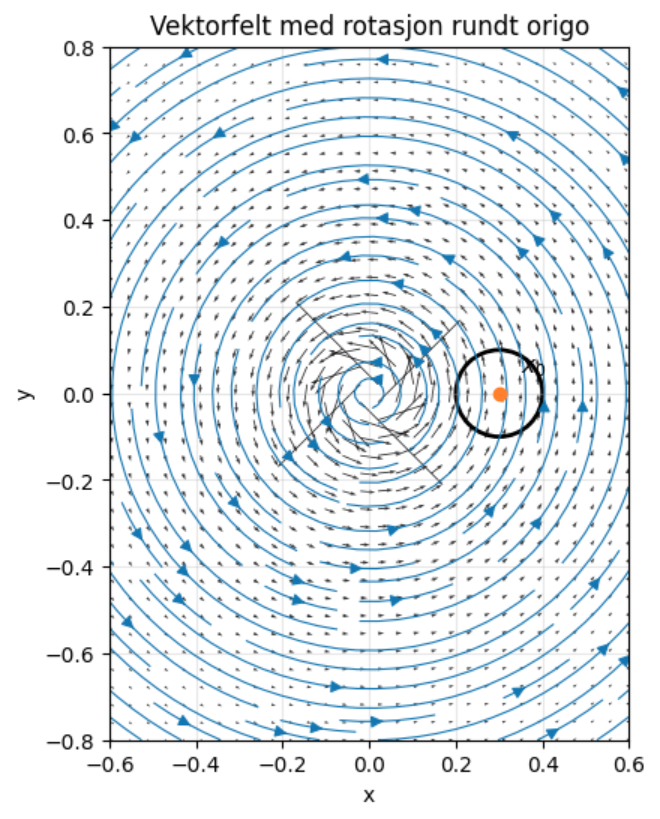
\includegraphics[width=0.6\linewidth]{Fig/fig_rotasjonsFritt.png}
    \caption{Figuren viser vektorfeltet $\vect{F}=(y,x,0)/r^2$ hvor $r^2=x^2+y^2.$ Dette vektorfeltet vil forårsake rotasjon rundt origo, som ikke er i definisjonsmengden ($D={\R^3 \setminus \{\vect{0}\}}$ Rotasjonen rundt et hvilket som helst punkt i definisjonesmengden (f.eks. det vilkårlig valgte oransje punktet) vil være null. Det betyr at ingen punkt vil sirkulere rundt dette punktet.}
    \label{fig:rotasjonsFritt}
\end{figure}

\begin{figure}[htpb]\centering
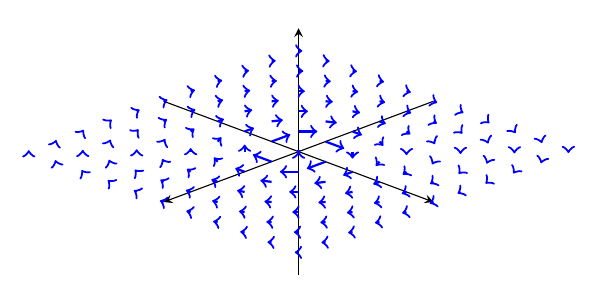
\begin{tikzpicture}[scale=1]
  \begin{axis}[
    view={135}{30},
    axis lines=center,
    xmin=-3, xmax=3,
    xtick = \empty,
    ytick= \empty,
    ztick = \empty,
    ymin=-3, ymax=3,
    zmin=-2, zmax=2,
    clip=false
  ]

  % Repeat quiver plot at multiple z levels
  \foreach \z in {0} {
    \addplot3[
      quiver={
        u={y/(x^2 + y^2 + 0.001)},
        v={-x/(x^2 + y^2 + 0.001)},
        w=0,
        scale arrows=0.25,
        every arrow/.append style={->, thick, blue}
      },
      domain=-3:3,
      y domain=-3:3,
      samples=11,
      samples y=11
    ]
    ({x}, {y}, {\z});
  }
  \end{axis}
\end{tikzpicture}
\caption{Vektorfelt $\vec{F}(x, y, z) = \dfrac{y\vec{i} - x\vec{j}}{x^2 + y^2}$}\label{fig:VF-irrot}
\end{figure}

\begin{prop}
 Hvis $f(x, y, z)$ har kontinuerlige deriverte av andre orden, så er $\mathrm{curl}(\nabla f) = \vect{0}$.
\end{prop}

\begin{oppsum}[Divergens av curl]\,
For et vektorfelt $\vect{F}(x,y,z)$ kan en enkelt vise at $\text{div }\cdot(\text{curl }\vect{F})=0.$ Dette følger av matematiske identiteter, og gir god fysisk mening: Det er ingen spredning i rotasjon, eller rotasjon i spredning. Uttrykt ved nabla-operatoren har vi altså at
\[\nabla\cdot\left(\nabla\times\vect{F}\right)=0.\]
\end{oppsum}
I og med at $\nabla$-operatoren kan betraktes sm en vektor, kan vi også ta prikkproduktet av den med seg selv. Dette gir den såkalte Laplace-operatoren.

\begin{defn}{Laplace}
For $f\colon \R^n\supseteq U \rightarrow \R$ defineres \emph{Laplace-operatoren}:
\[
\Delta f := \nabla^2 f := \text{div}(\nabla f)
\]
Så for to- og tredimensjonale rom får vi igjen de enklere formler
\begin{align*}
 \Delta f = \frac{\partial^2 f}{\partial^2 x} + \frac{\partial^2f}{\partial y^2} \quad \text{i 2D}, \qquad
 \Delta f = \frac{\partial^2 f}{\partial^2 x} + \frac{\partial^2f}{\partial y^2} +  \frac{\partial^2 f}{\partial^2 z} \quad \text{i 3D}
\end{align*}
\end{defn}
\begin{rem}{}
Alle differensialoperatorer beskrives her med hensyn til kartesiske koordinater. I andre koordinatsystemer ser de annerledes ut. For eksempel, Laplace er 
\[\Delta f = \frac{\partial^2 f}{\partial r^2} + \frac{1}{r}\frac{\partial f}{\partial r} + \frac{1}{r^2} \frac{\partial^2 f}{\partial^2 \varphi}\qquad \text{ i Polarkoordinater } (r,\varphi).\]
\end{rem}
Laplace-operatoren er viktig i formuleringen av bølgelikninger, som vi skal studere senere, når vi ser på partielle differensiallikninger. Et eksempel er Poisson-likningen; 
\[\Delta f=g\]
for to funksjoner $f$ og $g$. Merk at $\Delta f$ er et skalarfelt, i motsetning til $\nabla f, $ som er et vektorfelt.

\paragraph{Identiteter: }Det finnes massevis identiteter som knytter de klassiske differensialoperatorene sammen. I \Cref{app:diffop_ident} finnes det et overblikkstabell med de vanligste identiteter.
Det er mulig å definere vektorfelt ved hjelp av Sympy pakke og la dem beregne differensialoperatorene.

\begin{oppsum}{Differensialoperatorer og Sympy pakke}
\begin{minipage}{.9\columnwidth}
\begin{lst}{}
import sympy as sp

from sympy.vector import CoordSys3D

R = CoordSys3D('R')

v = 3*R.i + 4*R.j + 5*R.k

sp.curl(v)

sp.divergence(v)

sp.gradient(R.x*R.y*R.z)
\end{lst}
\end{minipage}
\end{oppsum}
\section{Linjeintegraler av vektorfelt}\label{sect:linint2}

Nå skal vi definere og studere linjeintegraler av vektorfelt. 
Disse integralene tar verdier i $\R$, ikke i flerdimensjonal rom.

\begin{defn}{Linjeintegral av vektorfelt}
La $\vect{F} \colon \R^n \rightarrow \R^n$ være et vektorfelt og $C$ en glatt kurve i $\R^n$ med parametrisering $\vect{r} \colon [a,b] \rightarrow \R^n$. Vi definerer \emph{linjeintegralet} av \( \vect{F} \) langs \( C \) som:
\begin{align}\label{defn:linjeint}
\int_C \vect{F} \cdot d\vect{r} = \int_a^b \vect{F}(\vect{r}(t)) \cdot \vect{r}\,'(t)\, dt \quad \text{ for } \vect{r}\,'=(r_1'(t),r_2'(t),\ldots, r_n'(t))^\top
\end{align}
Merk at integrasjonen virkelig er et skalarprodukt mellom vektorfeltet og differensialvektoren \( d\vect{r} \). Dermed er verdien til linjeintegralet igjen et tall!
\end{defn}
Mer konkret for vektorfeltet i tredimensjonalt rom:
\[
\vect{F}(x, y, z) = P(x, y, z)\, \vect{i} + Q(x, y, z)\, \vect{j} + R(x, y, z)\, \vect{k}
\]
og en glatt, tredimensjonal kurve gitt ved:
\[
\vect{r}(t) = x(t)\, \vect{i} + y(t)\, \vect{j} + z(t)\, \vect{k}, \quad a \leq t \leq b
\]
Setter vi formlene inn i \eqref{defn:linjeint} så er linjeintegralet av \( \vect{F} \) langs \( C \) gitt som:
\begin{align*}
&\int_C \vect{F} \cdot d\vect{r} = \int_a^b \vect{F}(\vect{r}(t)) \cdot \vect{r}\,'(t)\, dt \quad \text{ for } \vect{r}\,'=(x'(t),y'(t),z'(t))^\top \\=&\int_a^b P(x(t),y(t),z(t)) \cdot x'(t) + Q(x(t),y(t),z(t))\cdot y'(t) + R(x(t),y(t),z(t)) \cdot z'(t)\, dt
\end{align*}
\begin{oppsum}{Linjeintegral av vektorfelt vs linjeintegraler ved buelengde}
Alternativt kan linjeintegralet skrives som et integral med hensyn på buelengde:
\[
\int_C \vect{F} \cdot d\vect{r} = \int_C \vect{F} \cdot \vect{t}\, ds
\]
hvor \( \vect{t}(t) = \frac{\vect{r}\,'(t)}{\|\vect{r}\,'(t)\|} \) er enhetstangentvektoren.
Begge former er ekvivalente, men vi bruker vanligvis den første, da den er enklere å regne med.
\end{oppsum}
\begin{rem}{Forskjellige Linjeintegraler}
Merk at linjeintegraler (med hensyn til buelengde) ser relativt lik ut som linjeintegraler av vektorfelt. De kan skilles ved et blikk på integrator:
\begin{align*}
\text{Linjeintegral ved buelengde} \quad \int_C f \, {\color{red}ds}\\
\text{Linjeintegral for vektorfelt} \qquad \int_C \vect{F} {\color{red} \cdot \, d\vect{r}}  
\end{align*}
\end{rem}

\begin{eks}{}
Beregn
\[
\int_C \vect{F} \cdot d\vect{r}, \quad \text{hvor } \vect{F}(x, y, z) = xz\, \vect{i} - yz\, \vect{k}
\]
og \( C \) er linjesegmentet fra \( (-1, 2, 0) \) til \( (3, 0, 1) \).
\end{eks}

\begin{oppsum}{Regneregler for linjeintegral av vektorfelt og omvendt retning}
De vanlige regneregeler for summer \eqref{lin_int_linear} og linjer som er sammensatt av glatte stykker \eqref{lin_int_add} gjelder for linjeintegraler av vektorfelt. Regelene for integral av omvendt retning fra tidligere kapittel er ikke riktig lengre!

En nyttig egenskap ved linjeintegraler av vektorfelt er at hvis vi bruker omvendt orientering på kurven, endres fortegnet til integralet:
\[
\int_{-C} \vect{F} \cdot d\vect{r} = - \int_C \vect{F} \cdot d\vect{r}
\]
Dette gir mening siden integralet kan uttrykkes som sum av komponentintegraler og retningen bestemmer fortegnet på disse.
\end{oppsum}

Hovedanvendelsen av linjeintegraler er å beregne arbeidet som utføres på et objekt i et kraftfelt. Hvis et objekt beveger seg langs en kurve $C$ gjennom et kraftfelt $\vect{F}$, kan vi beregne det totale arbeidet som utføres av kraftfeltet ved å dele kurven $C$ opp i små biter.  
Arbeidet\footnote{Siden vi skriver $A$ for areal bruker vi har $W$ for arbeid som det engelske work.} $dW$ som gjøres på hver liten bit er tilnærmet gitt ved
\[
dW = \vect{F} \cdot \vect{t} \, ds = \vect{F} \frac{\vect{r}'(t)}{\|\vect{r}'(t)\|} \|\vect{r}'(t)\| \, dt = \vect{F} \cdot \vect{r}'(t) \, dt.
\]
Som vanlig summerer vi alle de små bidragene og tar grensen når lengden av bitene går mot null, noe som gir et integral.
\begin{defn}{Arbeid}\label{defn:arbeid}
La $\vect{F}$ være et vektorfelt og $C$ en kurve definert ved en vektorfunksjon $\vect{r}(t)$. Da er arbeidet utført av $\vect{F}$ på et objekt som beveger seg langs $C$ gitt ved
\[
\text{Arbeid} = \int_C \vect{F} \cdot d\vect{r} = \int_a^b \vect{F}(\vect{r}(t)) \cdot \vect{r}'(t) \, dt.\] 
\end{defn}

\begin{eks}{}
Hva er arbeidet som utføres av gravitasjonskraften
\[
\vect{F} = \frac{-1}{\lVert\vect{r}\rVert^2} \cdot \frac{\vect{r}}{\lVert \vect{r}\rVert} \text{  langs en sirkel rundt origo?}
\]
Siden radius ikke er spesifisert, bruker vi en variabel $R$ for radius og dermed er en parametrisering gitt som:
\[
\vect{r}(t) = R \cos(t) \vect{i} + R \sin(t) \vect{j}, \quad 0\leq t\leq 2\pi
\]
Merk at $\vect{F}$ er uttrykt som funksjon av $\vect{r}$. Vi bruker formel for arbeid-formelen:
\[
W = \int_0^{2\pi} \vect{F}(\vect{r}(t))(\vect{r}'(t))\, dt= \int_0^{2\pi}\frac{-1}{\lVert\vect{r}\rVert^2} \cdot \frac{\vect{r}}{\lVert \vect{r}\rVert}(\vect{r}'(t))\,dt
\]
La oss nå forenkle hver komponent:
\begin{align*}
\lVert\vect{r}\rVert^2 = R^2 (\cos^2(t) + \sin^2(t)) = R^2 
& &\Rightarrow \frac{\vect{r}(t)}{\lVert \vect{r}(t)\rVert} = \frac{1}{R}(\cos(t)\vect{i}+\sin(t)\vect{j})\\
\vect{r}'(t)=-R\sin(t)\vect{i}+R\cos(t)\vect{j}
\end{align*}
Nå setter vi alt inn i formelen for arbeid og får:
\begin{align*}
W &= -\frac{1}{R} \int_0^{2\pi} (\cos(t) \vect{i} + \sin(t) \vect{j}) \cdot (-\sin(t) \vect{i} + \cos(t) \vect{j})\, d t\\
 &= -\frac{1}{R} \int_0^{2\pi} [- \cos(t) \sin(t) +  \sin(t) \cos(t)] \dd{t}
= -\frac{1}{R} \int_0^{2\pi} 0 \dd{t} = 0
\end{align*}
\textbf{Alternativ:} Bevegelsen skjer langs en sirkel med posisjonvektor $\vect{r}(t)$, og hastighetsvektoren (tangenten) er alltid vinkelrett på $\vect{r}$. Dermed er skalarproduktet $\vect{F} \cdot d \vect{r} = 0$, siden kraften peker radielt og bevegelsen er tangentiell. Derfor er arbeidet null.
\end{eks}

%
%
%
\subsection*{Analysens fundamentalteorem for linjeintegraler}

Husk analysens fundamentalteorem for vanlige funksjoner:
\begin{align}\label{ana_fun_thm}
\int_a^b F'(x)\, dx = F(b) - F(a).
\end{align}
Noe tilsvarende gjelder for linjeintegraler og gradienter av funksjoner.

\begin{thm}[Fundamentalt Teorem for Linjeintegraler]\label{funthm_linjeint}
Anta at \( C \) er en glatt kurve gitt ved \( \vect{r}(t) \), \( a \leq t \leq b \), og at \( f \) er en funksjon slik at \( \nabla f \) er kontinuerlig på \( C \). Så er:
\[
\int_C \nabla f \cdot d\vect{r} = f(\vect{r}(b)) - f(\vect{r}(a))
\]
Her representerer \( \vect{r}(a) \) startpunktet og \( \vect{r}(b) \) sluttpunktet på kurven \( C \).
\end{thm}

\begin{proof}[Bevis (skisse)]
Vi antar at vi arbeider i tre dimensjoner. Start med å beregne:
\[
\int_C \nabla f \cdot d\vect{r} = \int_a^b \nabla f(\vect{r}(t)) \cdot \vect{r}'(t)\, dt
\]
Ved kjerneregelen:
\[
= \int_a^b \left(
\frac{\partial f}{\partial x} \frac{dx}{dt} +
\frac{\partial f}{\partial y} \frac{dy}{dt} +
\frac{\partial f}{\partial z} \frac{dz}{dt}
\right)\, dt
= \int_a^b \frac{df}{dt}\, dt \stackrel{\eqref{ana_fun_thm}}{=} f(\vect{r}(b)) - f(\vect{r}(a))\qedhere
\]
\end{proof}

Det betyr at linjeintegraler av vektorfelt beregnes kjempelett dersom feltet er konservativt og en potensial er kjent:
\begin{eks}{}
Evaluer:
\[
\int_C \nabla f \cdot d\vect{r}, \quad \text{der } f(x, y, z) = \cos(\pi x) + \sin(\pi y) - xyz
\]
og \( C \) er en hvilken som helst kurve fra punktet \( (1, \frac{1}{2}, 2) \) til \( (2, 1, -1) \). Så er
\[
\int_C \nabla f \cdot d\vect{r}=f(2, 1, -1) - f\left(1, \tfrac{1}{2}, 2\right)=(1+0+2)-(-1+1-1)=2
\]
\end{eks}
Det viktigste å merke seg er at for slike linjeintegraler spiller stien ingen rolle – det er kun start- og sluttpunkt som avgjør resultatet.
\newpage
\begin{defn}{}
La \( \vect{F} \) være et kontinuerlig vektorfelt i en mengde \( D \). Anta at $C$ er en kurve i $D$ parametrisert med $\vect{r}$. Vi sier  \( \int_C \vect{F} \cdot d\vect{r} \) er \emph{uavhengig av sti} hvis det samme verdien oppnås for enhver kurve $\tilde{C} \subseteq D$ med samme start- og sluttpunkt som $C$. 
\end{defn}

Spørsmålet er nå om vi kan karakterisere integraler som er uavhengig av sti. Det er hensiktsmessig å introdusere noen navner for spesielle mengder og kurver når vi er interessert i integraler uavhengig av sti.

\begin{minipage}{7cm}
\begin{defn}{Egenskaper til kurver}
 En kurve \( C \) er \begin{itemize}
 \item \textbf{lukket} hvis start- og sluttpunkt er like.
 \item \textbf{enkel} hvis den ikke krysser seg selv.
 \end{itemize}
\end{defn}
\end{minipage}%
% 
\begin{minipage}{7cm}
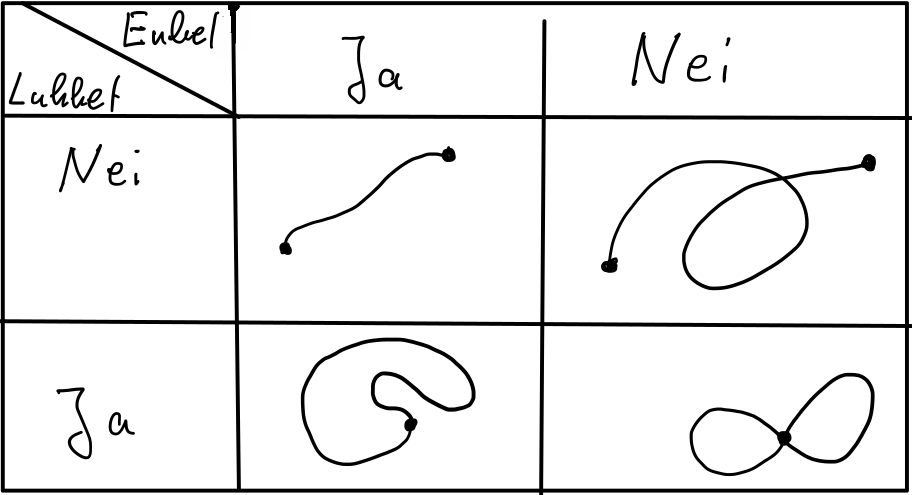
\includegraphics[width=7cm]{Fig/lukket_enkelt_kurver.png}
\end{minipage}

Vi skal møte lukkete og enkle kurver og linjeintegraler langs dem ofte siden de utgjør randen til enkle områder i planet.
 \begin{defn}{Egenskaper til mengder i $\R^n$}
 En mengde \( D \) kaller vi 
 \begin{itemize}
 \item \textbf{åpen} hvis den ikke inkluderer noen av sine randpunkter.
 \item \textbf{stjerneformet} hvis det finnes et punkt $\star \in D$ slik at for alle andre punkter $P \in D$ linjestykken mellom $\star$ of $P$ ligger fullstendig i $D$. Punkten $\star$ kaller man også \emph{stjernepunkt} for $D$.
\end{itemize}
\end{defn}

\begin{figure}[htpb]\centering
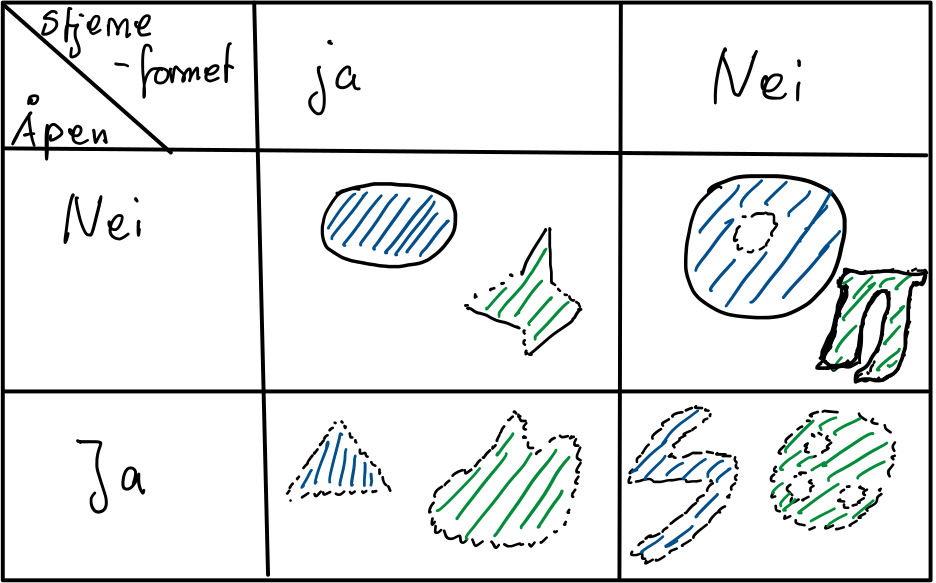
\includegraphics[width=12cm]{Fig/stjerneformet_mengde.png}
\caption{Tabellen viser to eksempler av mengder (blå og grønn) som oppfyller egenskapene. Stiplete linjer betyr at punktene ikke er med.}
\end{figure}
Vanligvis er stjernepunkter ikke unik, dvs. hvis et punkt er stjernepunkt for en mengde $D$ finnes det vanligvis også mange andre punkter som er stjernepunkter for $D$.
%
\begin{oppsum}{Fakta om konservative vektorfelt og linjeintegraler}
La $\vect{F}$ være et kontinuerlig vektorfelt på en mengde $D$.
\begin{enumerate}
    \item Hvis \( \vect{F} = \nabla f \) (dvs. vektorfeltet er konservativt), så er \( \int_C \vect{F} \cdot d\vect{r} \) uavhengig av sti. 
    \item Hvis $D$ er åpen og stjerneformet, og integralet er uavhengig av sti, så er \( \vect{F} \) konservativ.
    \item \( \int_C \vect{F} \cdot d\vect{r} = 0 \) for alle lukkede kurver \( C \) i \(D\) hvis og bare hvis  \( \int_C \vect{F} \cdot d\vect{r} \) er uavhengig av sti.
\end{enumerate}
\textbf{OBS:} På åpne og stjerneformete mengder er linjeintegraler av vektorfelt uavhengig av sti hvis og bare hvis vektorfeltet er konservativt.
\end{oppsum}

%
%
%
\section{Konservative Vektorfelt og Potensialer}\label{sect:konservativ}

Dersom et vektorfelt \( \vect{F} \) er konservativt, da er linjeintegralet \( \int_C \vect{F} \cdot d\vect{r} \) uavhengig av stien. 
Det betyr at vi enkelt kan evaluere linjeintegralet dersom vi kan finne en potensialfunksjon for \( \vect{F} \). 
Vi skal altså se på to spørsmål:
\begin{enumerate}
    \item Hvordan bestemmer vi om et vektorfelt er konservativt?
    \item Hvis et vektorfelt er konservativt, hvordan finner vi en potensialfunksjon?
\end{enumerate}

%
\subsection*{For to dimensjoner}
Vi begynner med to-dimensjonale vektorfelt. 
Det neste teoremet gir oss et praktisk test om noen vektorfelt er konservativt.

\begin{thm}\label{thm:kons_stjern_2D}
La \( \vect{F} = P\, \vect{i} + Q\, \vect{j} \) være et vektorfelt definert på en \textbf{åpen og stjerneformet} mengde \( D \). Dersom \( P \) og \( Q \) har kontinuerlige førstepartialderiverte på \( D \), og
\[
\frac{\partial P}{\partial y} = \frac{\partial Q}{\partial x}
\]
så er \( \vect{F} \) konservativt.
\end{thm}

\begin{eks}{}
Bestem om følgende vektorfelt er konservative:
\begin{itemize}
    \item[(a)] \( \vect{F}(x, y) = (x^2 - yx)\, \vect{i} + (y^2 - xy)\, \vect{j} \)
    \item[(b)] \( \vect{F}(x, y) = (2xe^{xy} + x^2 y e^{xy})\, \vect{i} + (x^3 e^{xy} + 2y)\, \vect{j} \)
\end{itemize}
\end{eks}

\begin{eks}{Moteksempel for konservative felt} \label{eks:moteks_konserv}
Betrakt vektorfeltet 
\[
\vect{F} = \frac{1}{x^2 + y^2}(-y, x)
\text{ på } D = \mathbb{R}^2 \setminus \{(0, 0)\} = \{(x, y) \in \mathbb{R}^2 \mid (x, y) \ne (0, 0)\}.
\]
Er vektorfeltet $\vect{F}$ konservativt?
\begin{align*}
P = \frac{-y}{x^2 + y^2} \qquad \text{ og } \qquad Q = \frac{x}{x^2 + y^2},
\\
P_y = \frac{(-1)(x^2 + y^2) - (-y)(2y)}{(x^2 + y^2)^2} 
= \frac{-x^2 - y^2 + 2y^2}{(x^2 + y^2)^2} 
= \frac{y^2 - x^2}{(x^2 + y^2)^2}.\\
Q_x = \frac{(x^2 + y^2) - (x)(2x)}{(x^2 + y^2)^2} 
= \frac{x^2 + y^2 - 2x^2}{(x^2 + y^2)^2} 
= \frac{y^2 - x^2}{(x^2 + y^2)^2}.
\end{align*}
Dermed $P_y = Q_x$. Likevel skal vi vise at $\vect{F}$ ikke er konservativt. La oss inegrere langs enhetssirkel $C$, parametrisert ved
\[
\vect{r}(t) = (\cos t, \sin t), 
\quad \vect{r}'(t) = (-\sin t, \cos t), \quad 0 \leq t \leq 2\pi.
\]
Integralet av $\vect{F}$ langs $C$ er
\begin{align*}
\int_C \vect{F} \cdot d\vect{r} &= 
\int_0^{2\pi} \vect{F}(\vect{r}(t)) \cdot \vect{r}'(t)\, dt
= \int_0^{2\pi} 
\begin{bmatrix}
\frac{-\sin t}{\cos^2 t + \sin^2 t}\\
\frac{\cos t}{\cos^2 t + \sin^2 t}
\end{bmatrix}
\cdot \begin{bmatrix}-\sin t\\ \cos t\end{bmatrix}\, dt
\\
&= \int_0^{2\pi} \begin{bmatrix}-\sin t\\ \cos t\end{bmatrix} \cdot \begin{bmatrix}-\sin t\\ \cos t\end{bmatrix}\, dt 
= \int_0^{2\pi} \sin^2 t + \cos^2 t\, dt 
= \int_0^{2\pi} dt 
= 2\pi \ne 0.
\end{align*}
Siden vi har funnet en lukket kurve der integralet av $\vect{F}$ ikke er null, kan ikke $\vect{F}$ være konservativt.
\end{eks}

Hvis vi ønsker å beregne en potensialfunksjon (for eksempel fordi vi ha funnet ut at vektorfeltet er konservativt!) kan vi gjøre det følgende.

\begin{oppsum}{Hvordan finne en potensialfunksjon?}
Anta at \( \vect{F} = P\, \vect{i} + Q\, \vect{j} \) er konservativ. Da finnes en funksjon \( f(x, y) \) slik at:
\[
\nabla f = \vect{F} \Rightarrow \frac{\partial f}{\partial x} = P,\quad \frac{\partial f}{\partial y} = Q
\]
\begin{enumerate}
\item[1.] Integrer \( P \) med hensyn på \( x \), eller \( Q \) med hensyn på \( y \):
\[
f(x, y) = \int P(x, y)\, dx \quad \text{eller} \quad f(x, y) = \int Q(x, y)\, dy
\]
Anta for nå at vi integrerer $P$. 

\begin{minipage}{.9\columnwidth}
\begin{rem}{}
     Integrasjonskonstanten er  avhengig av variablen (se \Cref{sect:dobbelint}). Dvs. $\int P(x, y)\, dx = \ldots + g(y)$ hvor $g$ er konstant avhengig av $y$.
\end{rem}
\end{minipage}
\item[2.] Beregn $\partial_y \int P(x, y)\, dx$.
\item[3.] Den deriverte fra 2. må være lik $Q(x,y)$ så vi få uttrykk for $g'(y)$. 
\item[4.] Beregn $g(y)= \int g'(y)\, dy$.
\item[5.] Sett sammen for å få potensial $f(x,y)$.
\end{enumerate}
\end{oppsum}

\begin{eks}{Feltet som blir konservativ på mindre området}
Bestem om vektorfelt $\vect{F}(x,y) = \frac{-y\vect{i}+x\vect{j}}{x^2+y^2}$ på det \textit{høyre halvplanet},
\[
D = \{(x, y) \in \mathbb{R}^2 \mid x > 0\}.
\] er konservative, og finn i så fall en potensialfunksjon.

I moteksempel tidligere har vi vist at $\vect{F}$ tilfredsstiller $P_y = Q_x$. Videre er $D$ stjerneformet. Dermed, ifølge \Cref{thm:kons_stjern_2D}, er $\vect{F}$ konservativt.

La oss finne en potensialfunksjon $f \colon D \to \mathbb{R}$, som må tilfredsstille
\[
f_x = P = \frac{-y}{x^2 + y^2}, \quad f_y = Q = \frac{x}{x^2 + y^2}.
\]
Ved å bruke den andre ligningen får vi
\[
f = \int Q\, dy = \int \frac{x}{x^2 + y^2}\, dy.
\]
Siden $x \ne 0$ i domenet, kan vi skrive
\[
\int \frac{x}{x^2 + y^2}\, dy = \int \frac{1}{1 + \left(\frac{y}{x}\right)^2} \, \frac{dy}{x} = \arctan\left(\frac{y}{x}\right) + g(x),
\]
hvor $g(x)$ er en funksjon av $x$. Deriverer vi med hensyn på $x$, får vi:
\[
\frac{\partial f}{\partial x}(x,y) = \frac{\partial}{\partial x} \left[\arctan\left(\frac{y}{x}\right)\right] + g'(x) 
= \frac{1}{1 + \left(\frac{y}{x}\right)^2} \cdot \left(-\frac{y}{x^2}\right) + g'(x) 
= \frac{-y}{x^2 + y^2} + g'(x).
\]
Ved å sammenligne dette med den første ligningen $f_x = P = \frac{-y}{x^2 + y^2}$, får vi
\[
\frac{-y}{x^2 + y^2} + g'(x) = \frac{-y}{x^2 + y^2} \quad \Rightarrow \quad g'(x) = 0 \quad \Rightarrow \quad g(x) = C,
\]
hvor $C$ er en konstant, med andre ord $f(x,y)=\arctan (\tfrac{x}{y})$ er en potensial for $\vect{F}$ på $D$.\footnote{Geometrisk tolkning: $f(x, y) = \arctan\left(\frac{y}{x}\right)$ måler vinkelen i polarkoordinater. 

Vinkelfunksjonen kan ikke defineres kontinuerlig på det punkterte planet $\mathbb{R}^2 \setminus \{(0, 0)\}$, fordi vinkelen må hoppe plutselig med $2\pi$ etter én runde rundt origo. Derimot kan vinkelfunksjonen defineres kontinuerlig på små områder som ikke omfatter origo. Det forklarer linjeintegralet 
\[
\int_C \vect{F} \cdot d\vect{r} = 2\pi
\]
langs enhetsirkelen, som vi beregnet i moteksempel. Ifølge den fundamentale setningen for linjeintegraler summerer dette integralet opp endringene i vinkel når vi beveger oss langs sirkelen $C$. Etter én fullstendig omdreining summerer vinkelendringene seg til $2\pi$.}
\end{eks}

\begin{rem}{Og moralen er... }
Det er avhengig av mengden vektorfeltet er definert på om den er konservativt (dvs. tilatter en potensial).
Hvis vi endrer mengden kan vektorfeltet blir konservativt selv om den ikke var det tidligere!
\end{rem}
\begin{figure}[htpb]
    \centering
    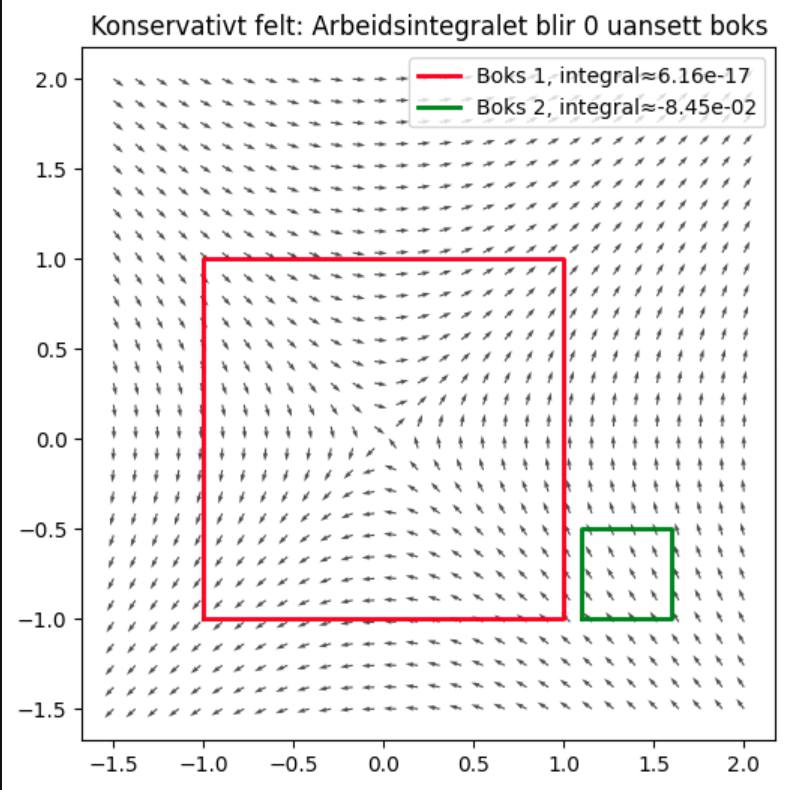
\includegraphics[width=0.5\linewidth]{Fig/konservativt.png}
    \caption{Figuren viser vektorfeltet
    \(\vect{F}(x,y)=(y,x)/r\) hvor $r=\sqrt{x^2+y^2}.$ En kan her vise at det finnes en potensialfunksjon, og $\vect{F}$ er derfor konservativt. Det medfører at uansett om vi integrerer langs den røde (store) eller grønne (lille) lukkede sløyfen (eller en hvilken som helst annen lukket kurve) så vil arbeidsintegralet bli null.}
    \label{fig:placeholder}
\end{figure}

\subsection*{I tre-dimensjoner}
I tre dimensjoner kan vi beregne en potensial liknende som i to dimensjoner, men det er vert å sjekke først at vektorfeltet faktisk er konservativ. 

\begin{oppsum}{Fakta om konservative vektorfelt og rotasjon}
\begin{enumerate}
    \item Hvis $\vect{F}$ er et konservativt vektorfelt, så er $\text{curl}(\vect{F}) = \vect{0}$.
    \item Hvis $\vect{F}$ er definert på en stjerneformet mengde (f.eks. hele $\mathbb{R}^3$), har kontinuerlige første ordens partiell deriverte, og $\text{curl}(\vect{F}) = \vect{0}$, da er $\vect{F}$ konservativt.
\end{enumerate}
\end{oppsum}
Dermed kan vi teste om et vektorfelt er konservativ ved å beregne curl! 

\begin{eks}{}
Gitt $\vect{F}(x,y,z) = x^2y \vect{i} + xyz \vect{j} - x^2y^2 \vect{k}$.
Da er:
\[
\text{curl } \vect{F} = -(2x^2y + xy) \vect{i} + 2xy^2 \vect{j} + (yz - x^2) \vect{k} \neq \vect{0}
\]
Altså, vektorfeltet er ikke konservativt.
\end{eks}
%
Gitt at \( \vect{F} = P\, \vect{i} + Q\, \vect{j} + R\, \vect{k} \) er konservativt, så finnes en funksjon \( f(x, y, z) \) slik at:
\[
\nabla f = \vect{F} \Rightarrow \frac{\partial f}{\partial x} = P, \quad \frac{\partial f}{\partial y} = Q, \quad \frac{\partial f}{\partial z} = R
\]
Fremgangsmåten med integrasjon, integrasjonskonstanten som er avhengig av de andre variabler osv. er lik som i to dimensjoner (men krever enda mer innsats).

%\begin{eks}{}
%Finn en potensialfunksjon for:
%\[
%\vect{F} = 2xy^3 z^4\, \vect{i} + 3x^2 y^2 z^4\, \vect{j} + 4x^2 y^3 z^3\, \vect{k}
%\]
%\end{eks}

\begin{eks}{}
Finn en potensial for 
\[\mathbf{F}(x,y,z)=\underbrace{(\sin(yz)+y-z)}_{P(x,y,z)}\vect{i}+\underbrace{(xz\cos(yz)+x)}_{Q(x,y,z)}\vect{j}+\underbrace{(xy\cos(yz)-2z-x)}_{R(x,y,z)}\vect{k}\]
\textbf{Metode I: Vanlig fremgangsmåte (sikker og uproblematisk)} Vi regner
\begin{itemize}
\item $f(x,y,z)=\int P(x,y,z)dx = x\sin(yz)+xz-xz+C(y,z)$
\item $\partial_y f(x,y,z) = Q(x,y,z)$ dvs. $xz\cos (yz)+x+C_y(y,z)=xz\cos(yz)+x$
\item Dermed $C_y(y,z)=0$ dvs. $C(y,z)=D(z)$ og $f(x,y,z)=xy\sin (yz)+xy-xz+D(z)$
\item $f_z(x,y,z)=R(x,y,z)$ dvs. $xy\cos(yz)-x+D_z(z)=xy\cos(yz)-x-2z$ gir $D_z(z)=2z$
\item Dermed $D(z)=-z^2$ og $f(x,y,z)=x\sin(yz)+xy-z^2-xz$.
\end{itemize}
\textbf{Metode II: Juksemetode (OBS: Fremgangsmåten er ikke sikker og behøver at man tester resultatet!!!)}
Vi lager integralene $\int P(x,y,z)dx, \int Q(x,y,z)dy$ og $\int R(x,y,z)dz$, oppsummer alle bidrag man får, men noter hver uttrykk som finnes dobbelt eller flere ganger bare en gang:
\begin{align*}
x\sin(yz)+xy-xz &&\\
x \sin (yz)+xy  & \Rightarrow& f(x,y,z)=x\sin (yz)+xy-z^2-xz\\
x\sin (yz)-z^2-xz &&
\end{align*}
Merk at resultatet samsvarer med funksjonen vi fikk fra Metode 1. Det gikk bra i dette tilfelle, men vanligvis må man sjekke og bruke den vanlige metoden hvis det ikke går opp.
\end{eks}

%
%
%
\section{Fluks og fluksintegral i 2D}\label{sect:fluks2d}

I \Cref{defn:arbeid} har vi definert for en kurve $C$ parametrisert via $\vect{r}$:
\[
\text{Arbeid utført av } \vect{F} \text{ langs } C = \int_C \vect{F} \cdot d\vect{r} = \int_C \vect{F} \cdot \hat{\vect{t}} \, ds
\]
hvor $\hat{\vect{t}}$ er enhetstangentenvektor (se \Cref{defn:enhetstangent}). Dermed kan vi forstå $\vect{F} \cdot \hat{\vect{t}}$ som bidrag vektorfeltet gir i retning av kurven. Vi lurer nå om bidrag av vektorfeltet som krysser kurven.

\begin{defn}{}
Anta at $\vect{r}(t)=x(t)\vect{i}+y(t)\vect{j}$ er en deriverbar kurve. 
En kan da vise at en \emph{normalvektor} $\vect{n}(t)$ til kurven $\vect{r}(t)$ er 
\[\vect{n}(t)=y'(t)\vect{i}-x'(t)\vect{j}\]
En \emph{enhetsnormalvektor} $\hat{\vect{n}}$ til $\vect{r}(t)$ må da være 
\begin{align}\label{enhetsnormal}
\hat{\vect{n}}(t)=\frac{\vect{n}}{|\vect{n}]}= \frac{y'(t)}{\sqrt{(x'(t))^2+(y'(t)^2)}}\vect{i}-\frac{x'(t)}{\sqrt{(x'(t))^2+(y'(t)^2)}}\vect{j}\end{align}
\end{defn}
%
At \(\vect{n}\) er en normalvektor kan man lett innse ved å huske på at \(\vect{t}(t):=\vect{r}'(t)=x'(t)\vect{i}+y'(t)\vect{j}\) er tangentvektor. Ettersom $\vect{n}\cdot\vect{t}=0$ så ser man at disse står normalt på hverandre. Altså er $\vect{n}$ normal til banen $\vect{r}(t)$.
\begin{defn}{Fluksintegral}
La $\vect{F}(x,y)=P(x,y)\vect{i}+Q(x,y)\vect{j}$ være et vektorfelt og $C$ en kurve parametrisert via $\vect{r} $. Vi velger enhetsnormalvektor $\vect{n}$ til kurven. Linjeintegralet av $\vect{F} \cdot \vect{n}$ over $C$ kalles \emph{fluks} eller \emph{fluksintegral} av $\vect{F}$ over $C$. I symboler:
\[
\text{Fluks av } \vect{F} \text{ over } C = \int_C \vect{F} \cdot \hat{\vect{n}}\, ds = \int P(x(t),y(t))y'(t)  - Q (x(t),y(t))x'(t) dt
\]
\end{defn}
%
Før vi fortsetter, la oss diskutere normalvektorer til kurver i 2D. Fluksintegralet er avhengig av et valg: 
Som \Cref{fig:orientering2D} viser, finnes det alltid to mulige retninger for en normalvektor til en kurve.
\begin{figure}[htpb]
  \centering

  % First subfigure
  \begin{subfigure}[b]{0.45\textwidth}
    \centering
    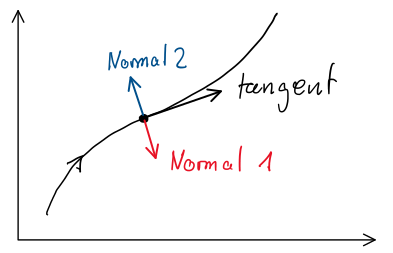
\includegraphics[width=\textwidth]{Fig/normal_2dkurve.png}
    \caption{To normaler, en som peker til venstre og en til høyre.}
    \label{fig:sub1}
  \end{subfigure}
  \hfill
  % Second subfigure
  \begin{subfigure}[b]{0.45\textwidth}
    \centering
    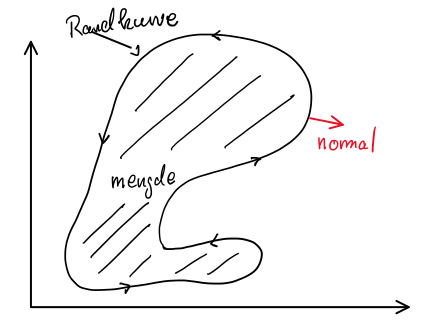
\includegraphics[width=\textwidth]{Fig/normal_orientering.png}
    \caption{Randkurven til et område. Området ligger til venstre av kurven}
    \label{fig:sub2}
  \end{subfigure}
  \caption{Orientering til normalvektorer og kurver som er randkurver til et området.}
  \label{fig:orientering2D}
\end{figure}
Vi må dermed velge en retning som normalen skal peke i (og alltid ville ha to muligheter for det). Det samme gjelder kurver som er lukket og er randkurver av en mengde (se \Cref{fig:sub2}). Her velger vi alltid orientering i henhold til \textit{høyrehåndsregelen}. Dermed kan vi slå fast følgende.

\begin{oppsum}{Standardorientering for kurver i 2D}
For en kurve $C$ med parametrisering $\vect{r}(t)$ er standardorientering for normalvektor at den peker til høyre (sett i retningen kurven går). Det er Normal 1 i \Cref{fig:sub1}.
Vektoren $\hat{\vect{n}}$ vi definerte i \eqref{enhetsnormal} er vektoren av lengde $1$ som peker til høyre.

Hvis $C$ er randkurven til et enkelt lukket området $D$ så skal vi alltid anta at $C$ er parametrisert slik at $D$ ligger til venstre av kurven. Vi sier at \( C \) har \emph{positiv orientering} i dette tilfellet og merker at enhetsnormalvektor $\vect{n}$ peker ut fra området (se \Cref{fig:sub2}).
\end{oppsum}
%
Vi skal vanligvis regne med standardorientering når vi snakker om fluksintegral.

\begin{eks}{Fluks over en linje}
Beregn fluksintegral av $\vect{F}(x,y)=2\vect{i}$ gjennom kurven fra $\vect{r}_1=3\vect{i}$ til $\vect{r}_2=\vect{3}j$ (med hensyn til standardorientering).

Først velger vi standardparametrisering for kurven som er gitt som $\vect{r}(t)=3(1-t)\vect{i}+3t\vect{j}, t \in [0,1]$. 
Dermed blir 
\[\hat{\vect{n}} = \frac{3 \vect{i}+3\vect{j}}{\sqrt{18}}, \quad \lVert \vect{r}'(t)\rVert = \sqrt{18}\]
Nå beregner vi fluksintegralet
\[\int_C \vect{F} \cdot \hat{\vect{n}}\, ds = \int_0^1 \vect{F}(\vect{r}(t))\cdot \hat{\vect{n}}(\vect{r}(t)) \,dt= \int_0^12\cdot 3 \, dt = 6\]
Hvis vi hadde brukt normalvektoren som peker i motsatt retning, altså $\hat{\vect{n}}_2=-\hat{\vect{n}}$, ville vi fått
\[\int_C \vect{F} \cdot \hat{\vect{n}}_2\, ds = -\int_C\vect{F} \cdot \hat{\vect{n}}\, ds =-6.\]
\end{eks}

\begin{rem}{Fluksintegral for omvendt orientering}
Merk at det er vilkårlig hvilken orientering av fluksen vi velger. Det viktige er bare at vi vet hvilket valg vi har gjort, slik at vi vet hvilken retning vektoren peker, og dermed hva som er positiv og negativ retning.
\end{rem}

%
\subsection*{Fysisk tolkning av fluks}
Tenk på $\vect{J}$ som et to-dimensjonalt strømningsfelt. Da representerer linjeintegralet den totale massestrømmen per tidsenhet som krysser kurven $C$ (f.eks. gjennom en tynn tank med dybde 1).
For et konstant felt $\vect{J}$ og et linjesegment $C$ med lengde $L$, er:
\[
\text{Massestrøm} = (\vect{J} \cdot \hat{\vect{n}})L
\]
Ved å dele kurven opp i små segmenter og summere bidragene får vi:
\[
\text{Total massestrøm over } C = \int_C \vect{J} \cdot \hat{\vect{n}} \, ds
\]
Den totale massestrømmen kaller vi da gjerne for \textit{fluksen} av $\vect{J}$ over $\textit{C}$. Strømtettheten $\vect{J}$ kan da kalles \textit{flukstettheten}. I elektromagnetismen er disse begrepene mye brukt. Kanskje oppleves de å være mer passende begreper i 3dimensjoner, hvor flukstettheten blir gjennomstrømningen \textit{per flate}, og ikke bare over en kurve $\textit{C}$.

\begin{eks}{Fluks av felt $F$}
Beregn fluksen av feltet 
\[
\vect{F} = \frac{x\vect{i} + y\vect{j}}{x^2 + y^2}
\]
gjennom en sirkel med radius $a$ og sentrum i origo, ved hjelp av:
\begin{enumerate}
\item Formel for $\vect{F} \cdot \hat{\vect{n}}$,
\item Parametrisering og differensialer.
\end{enumerate}

\textbf{Løsning a)}: I kulekoordinater kan vektorfeltet skrives som (prøv å skrive om!)
\[\vect{F}=\frac{1}{r}\hat{\vect{r}}.\]
Det blir da tydelig at feltet peker radialt utover, så $\vect{F}$ og $\hat{\vect{n}}$ har samme retning. Derfor er:
\[
\vect{F} \cdot \hat{\vect{n}} = |\vect{F}| = \frac{1}{\sqrt{x^2 + y^2}} = \frac{1}{a}
\]
Fluksen blir da:
\[
\int_C \vect{F} \cdot\hat{\vect{n}} \, ds = \int_C \frac{1}{a} \, ds = \frac{1}{a} \cdot (2\pi a) = 2\pi
\]

\textbf{Løsning b)}: Bruk parametrisering $x = a \cos t$, $y = a \sin t$, $t \in [0, 2\pi]$:
\begin{align*}
\text{Fluks} &= \int_0^{2\pi} \frac{x(t)\cdot a \cos(t) + y(t)\cdot a \sin(t) }{x(t)^2 + y(t)^2}  dt = \int_0^{2\pi} \frac{a^2 \cos^2 t + a^2 \sin^2 t}{a^2} \, dt \\ &= \int_0^{2\pi} 1 \, dt = 2\pi
\end{align*}
\textbf{Fysisk tolkning:}
Feltet 
\[
\vect{F} = \frac{x\vect{i} + y\vect{j}}{x^2 + y^2}
\]
representerer strøm fra en punktkilde i origo med styrke $2\pi$, og vi ser at fluksen gjennom enhver sirkel med sentrum i origo blir $2\pi$, uavhengig av radiusen.
\end{eks}



%
%
%
\section{Green's teorem}\label{sect:green}
Anta at \( C \) er en enkel, lukket kurve, og la \( D \) være området innesluttet av kurven. Det viser seg at det er en sammenheng mellom linjeintegraler over $C$ og dobbeltingetraler of $D$. 
Denne sammenhengen er kjent som \textit{Green's teorem}. Dette er det første av flere integralteorem\footnote{Analysens fundamentalteorem \eqref{ana_fun_thm} og dens generalisering for linjeintegraler \Cref{funthm_linjeint} er faktisk også integralteoremer av en lignende typ.} som vi skal bli kjent med i resten av dette kapitlet. 


\begin{thm}[Green's teorem]\label{thm:Green}
La \( C \) være en positivt orientert, stykkevis glatt, enkel, lukket kurve og \( D \) området innelukket av \( C \). Dersom \( \mathbf{F}(x,y) = P(x,y)\mathbf{i} + Q(x,y) \mathbf{j} \) har kontinuerlige første partialderiverte på \( D \) så gjelder 
\[
\int_C \mathbf{F} \cdot d\mathbf{r} = \iint_D \left( \frac{\partial Q}{\partial x} - \frac{\partial P}{\partial y} \right) dA.
\]
\end{thm}

\begin{rem}{}
Dersom $C$ er en lukket kurve bruker vi ofte symbolet "$\oint$" istedet for det vanlige "$\int$". Det er for å presisere at kurven er lukket.

Det er vanlig å si at \Cref{thm:Green} er et teorem om 2D-rotasjon fordi man kan forstå formelen slik at vektorfelt integrert over randen til et lukket området er lik arealintegral av rotasjonen i området. For å motivere det trenger vi en liten identifikasjon:

Husk at 2D-rom $\R^2$ kan identifiseres med $xy$-planet i 3D-rom. Med andre ord, hver vektor med to komponenter kan identifiseres ved en 3D vektor ved å anta at tredje komponent er lik $0$. Det samme for et et vektorfelt
\[\vect{F} (x,y)=P(x,y)\vect{i}+Q(x,y)\vect{j} \Rightarrow \hat{\vect{F}}(x,y,z):=P(x,y)\vect{i}+Q(x,y)\vect{j}+0\cdot \vect{k}.\]
Et eksempel for dette er feltet vi har sett på i \Cref{fig:rotasjonsFritt} (og det var grunn hvorfor det var tilstrekkelig å se på et 2D bildet!)

For 3D vektorfelt har vi definert rotasjonen og gitt interpretasjon at det beskriver hvordan det viser rotasjon rundt et punkt.
Hvis vi beregner nå
\[\mathrm{curl} (\hat{\vect{F}}) = \begin{bmatrix} \vdots \\ \frac{\partial Q}{\partial x}-\frac{\partial P}{\partial y}\end{bmatrix}\]
Så tredje komponent er akkurat det vi ser som integrand i Green's teorem. Defor kaller noen uttrykket $\mathrm{curl}(\hat{\vect{F}})\cdot \vect{k}$ også en 2D-curl (eller 2D rotasjon).

Interpretasjonen ville være nyttig for å knytte Green's \Cref{thm:Green} til Stokes'  integralteorem (\Cref{thm:stokes}) som vi skal se på senere.
\end{rem}

\begin{eks}{Vi verifiserer  \Cref{thm:Green} i et eksempel} \label{ex:greenveri}
For \( \mathbf{F}\) slik at \(P(x, y) = x \) og \( Q(x, y) = xy \), der \( D = \{(x,y) \in \R^2 \colon x^2 + y^2 \leq 1 \} \).

Vi gjør dette ved å evaluere begge sider i Greens teorem direkte. Randen av \( D \) er enhetsirkelen, som kan parameteriseres ved  
\( x = \cos t, \; y = \sin t, \; 0 \leq t \leq 2\pi \), og dermed:
\begin{align*}
\oint_{\partial D} \mathbf{F}\cdot\, d\mathbf{r} &=
\int_0^{2\pi} \left[(\cos t)(-\sin t) + \cos t \cdot \sin t \cdot \cos t\right] dt
\\ &= \int_0^{2\pi} \left[ -\cos t \sin t + \cos^2 t \sin t \right] dt
= \left[ \frac{\cos^2 t}{2} \right]_0^{2\pi} + \left[ -\frac{\cos^3 t}{3} \right]_0^{2\pi} = 0
\end{align*}
På den andre siden har vi:
\[
\iint_D \left( \frac{\partial Q}{\partial x} - \frac{\partial P}{\partial y} \right) \, dx\,dy
= \iint_D y \, dx\,dy,
\]
som forsvinner på grunn av symmetri. Dermed er Greens teorem verifisert i dette tilfellet.
\end{eks}
%
\begin{rem}{}
 Merk at arealintegral i \Cref{ex:greenveri} var mye enklere å evaluere enn linjeintegralet. Det viser hvordan man vanligvis bruker Greens teorem: Vi bytter areal med linjeintegral eller omvendt for å finne en enklere måte å beregne integraler.
\end{rem}
%
\begin{eks}{}
La \( C \) være trekanten med hjørner i \( (0,0),\ (1,0),\ (1,2) \), positivt orientert. Beregn
\[
\int_C \begin{bmatrix} xy\\ x^2 y^3\end{bmatrix} \cdot \, d\mathbf{r},
\]
La oss først identifisere delene:
\begin{align*}
P = xy, \quad Q = x^2 y^3
\\
\frac{\partial Q}{\partial x} = 2x y^3, \quad \frac{\partial P}{\partial y} = x
\Rightarrow \frac{\partial Q}{\partial x} - \frac{\partial P}{\partial y} = 2x y^3 - x
\end{align*}
Området $D$ parametriseres som i \Cref{ex:trekant_para}: \( 0 \leq x \leq 1,\ 0 \leq y \leq 2x \). 
Dermed 
\[
\oint_C \begin{bmatrix} xy\\ x^2 y^3\end{bmatrix} \cdot \, d\mathbf{r} \stackrel{\Cref{thm:Green}}{=} \iint_D (2x y^3 - x)\, dA = \int_0^1 \int_0^{2x} (2x y^3 - x)\, dy\, dx = \frac{4}{3}
\]
\end{eks}
\newpage

\begin{prop}[Greens teorem for fluks]
\label{green:fluks}
La \( D \subset \mathbb{R}^2 \) være et område der Greens teorem gjelder, og la \(C=  \partial D \) være dets rand. La \( \mathbf{F} = P\mathbf{i} + Q\mathbf{j} \) være et kontinuerlig deriverbart vektorfelt på \( D \). Da gjelder:
\[
\oint_{C} \vect{F} \cdot \vect{n} \, ds = \iint_D \operatorname{div} \vect{F} \, dA.
\]
\end{prop}

\begin{eks}{}
La \( \mathbf{F} = y^3\mathbf{i} + x^5\mathbf{j} \). Beregn fluksintegralet til \( \mathbf{F} \) rundt enhetskvadrat $Q$.  
Vi bruker Greens teorem for fluksintegraler \Cref{green:fluks}:
\[
\oint_{\partial Q} \mathbf{F} \cdot \mathbf{n} \, ds = \iint_Q \operatorname{div} \mathbf{F} \, dA,
\]
men \( \operatorname{div} \mathbf{F} = 0 \), og dermed er integralet lik null.
\end{eks}

%
\subsection{Utvidelse av Green's teorem ved oppdeling av områder}
Green's teorem gjelder ikke direkte for områder med hull. Men, ved å dele området og summere integralene kan vi vise at det fortsatt fungerer.

For eksempel, hvis vi har en ring mellom to sirkler, kan vi dele området i to og bruke Green's teorem på hver del. Grensekurver som går i motsatt retning kansellerer hverandre.
\begin{center}
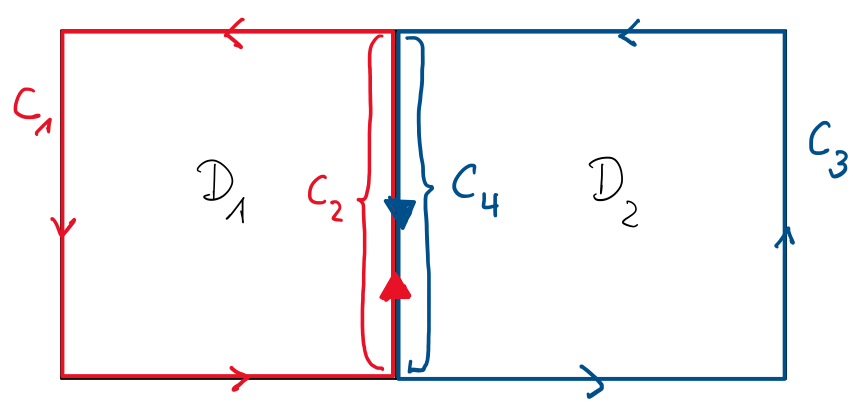
\includegraphics[width=8cm]{Fig/Green_del_sqrs.png}
\end{center}
Området \( D \) vil være \( D_1 \cup D_2 \), og vi minner om at symbolet \( \cup \) betegner union, altså at \( D \) består av både \( D_1 \) og \( D_2 \).

Den vertikale randen til \( D_1 \) består av \( C_1 \cup C_2 \), mens den vertikale randen til \( D_2 \) består av \( C_3 \cup (C_4) = C_3 \cup (-C_2)\). Begge disse grensene er positivt orientert – det vil si at mens vi beveger oss langs grensen, ligger det tilsvarende området alltid til venstre.
Til slutt kan vi tenke på hele den vertikale delen \( C \)  av randen som:
\[
C = (C_1 \cup C_2) \cup (C_3 \cup (-C_2)) = C_1 \cup C_2
\]
siden \( C_2\) og \( -C_2 \) vil kansellere hverandre. Det må vi forklare nå med hensyn til integralene.

Vi starter med følgende dobbeltintegral og deler det opp:
\[
\iint_D \left( \frac{\partial Q}{\partial x} - \frac{\partial P}{\partial y} \right)\, dA
= \iint_{D_1} \left( \frac{\partial Q}{\partial x} - \frac{\partial P}{\partial y} \right)\, dA
+ \iint_{D_2} \left( \frac{\partial Q}{\partial x} - \frac{\partial P}{\partial y} \right)\, dA
\]
Nå bruker vi Greens teorem på hver av integralene, og bruker samtidig at vi kan splitte linjeintegraler langs grensene:
\begin{align*}
\iint_D \left( \frac{\partial Q}{\partial x} - \frac{\partial P}{\partial y} \right)\, dA
&= \iint_{D_1} \left( \frac{\partial Q}{\partial x} - \frac{\partial P}{\partial y} \right)\, dA
+ \iint_{D_2} \left( \frac{\partial Q}{\partial x} - \frac{\partial P}{\partial y} \right)\, dA \\
&= \oint_{C_1 \cup C_2}\begin{bmatrix} P\\ Q\end{bmatrix} \cdot \, d\mathbf{r}
+ \oint_{-C_2 \cup (C_3)} \begin{bmatrix} P\\ Q\end{bmatrix} \cdot \, d\mathbf{r} \\
&= \oint_{C_1} \begin{bmatrix} P\\ Q\end{bmatrix} \cdot \, d\mathbf{r}
+ \oint_{C_2} \begin{bmatrix} P\\ Q\end{bmatrix} \cdot \, d\mathbf{r}
+ \oint_{-C_2}\begin{bmatrix} P\\ Q\end{bmatrix} \cdot \, d\mathbf{r}
+ \oint_{C_3} \begin{bmatrix} P\\ Q\end{bmatrix} \cdot \, d\mathbf{r}
\end{align*}
Nå bruker vi at:
\[
\oint_{-C_2} \begin{bmatrix} P\\ Q\end{bmatrix} \cdot \, d\mathbf{r} = -\oint_{C_2} \begin{bmatrix} P\\ Q\end{bmatrix} \cdot \, d\mathbf{r}
\]
Å endre orienteringen av en kurve i linjeintegraler med hensyn på \( dx \) og/eller \( dy \) endrer bare fortegnet på integralet. Om du vil: Vi integrerer det samme vektorfeltet over den samme grensen, men motsatt vei. Da får vi motsatt fortegn. Bidragene kansellerer derfor mot hverandre:
\begin{align*}
\iint_D \left( \frac{\partial Q}{\partial x} - \frac{\partial P}{\partial y} \right)\, dA
&= \oint_{C_1}\begin{bmatrix} P\\ Q\end{bmatrix} \cdot \, d\mathbf{r}
+ \oint_{C_2} \begin{bmatrix} P\\ Q\end{bmatrix} \cdot \, d\mathbf{r}
+ \oint_{C_3} \begin{bmatrix} P\\ Q\end{bmatrix} \cdot \, d\mathbf{r}
- \oint_{C_2}\begin{bmatrix} P\\ Q\end{bmatrix} \cdot \, d\mathbf{r} \\
&= \oint_{C_1} \begin{bmatrix} P\\ Q\end{bmatrix} \cdot \, d\mathbf{r} + \oint_{C_3}\begin{bmatrix} P\\ Q\end{bmatrix} \cdot \, d\mathbf{r}
\end{align*}
Sett sammen igjen linjeintegralene:
\[
\iint_D \left( \frac{\partial Q}{\partial x} - \frac{\partial P}{\partial y} \right)\, dA
= \oint_{C_1} \begin{bmatrix} P\\ Q\end{bmatrix} \cdot \, d\mathbf{r} + \oint_{C_3} \begin{bmatrix} P\\ Q\end{bmatrix} \cdot \, d\mathbf{r}
= \oint_{C_1 \cup C_3} \begin{bmatrix} P\\ Q\end{bmatrix} \cdot \, d\mathbf{r} = \oint_C \begin{bmatrix} P\\ Q\end{bmatrix} \cdot \, d\mathbf{r}
\]
Det viktige poenget her er at når vi deler opp et område slik vi gjorde ovenfor, så vil de delene av grensen som går i motsatt retning \emph{inni området} kansellere hverandre.

Denne innsikten er svært nyttig når vi skal håndtere områder med hull i.

Figur~\ref{fig:oppdeling} viser hvordan vi kan benytte denne innsikten. Området viser et domene $C_1$ med hull i ($C_2$). Ved å dele opp i to domener ser vi at Greens teorem tilslutt kan anvendes ved å se på både $C_1$ og $C_2$ som deler av randen til området. 
\begin{figure}[ht]
\centering
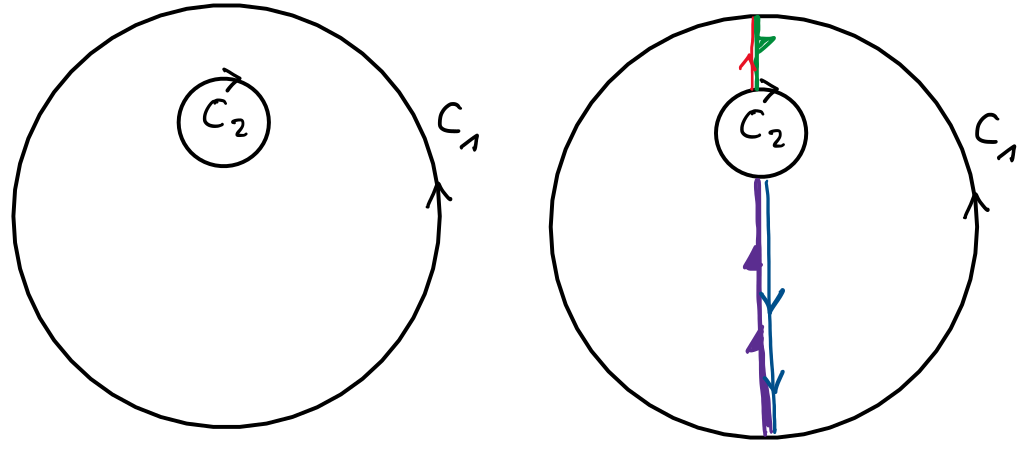
\includegraphics[width=12cm]{Fig/Green_del2_circles.png}
\caption{Oppdeling av en mengde for å anvende Green`s teorem.}
\label{fig:oppdeling}
\end{figure}

\begin{eks}{Green's teorem på en ring}
Beregn integralet
\[\oint_{\partial D} \left((\sin(x)-\frac{y^3}{3})\vect{i}+(\frac{x^3}{3}+\sin (y))\vect{j}\right)\cdot \, d\vect{r}\]
der $\partial D$ er positivt orientert og  området $D$ er ringen gitt i polarkoordinater ved ulikhetene
\[1\leq r \leq 2, 0 \leq \theta \leq 2 \pi\]
Vi kan bruke Green's teorem i utvidet form for å beregne integralet. Det gir oss
\begin{align*}
\oint_{\partial D} \left((\sin(x)-\frac{y^3}{3})\vect{i}+(\frac{x^3}{3}+\sin (y))\vect{j}\right)\cdot \, d\vect{r} &= \iint_D \left(x^2+ y^2) \right) dA\\
&=\int_0^{2\pi}\int_1^2 r^3\, dr d\theta = \int_0^{2\pi} \frac{15}{4}\, d\theta = \frac{15\pi}{2}
\end{align*}
\end{eks}

\begin{eks}{Vektorfelt på punktert planet}
Vi har sett i Eksempel 2.12 og 2.13, \Cref{eks:moteks_konserv}, på feltet 
\[\vect{F}(x,y) = \frac{-y\vect{i}+x\vect{j}}{x^2+y^2}, \qquad \text{ på }\quad  D:= \R^2 \setminus \{\vect{0}\}\]
Husk at
\begin{itemize}
\item når $S$ er en sirkel rundt origo (positiv orientering), så er $\oint_S \vect{F}\cdot d\vect{r}=2\pi$. 
\item hvis vi ser på feltet i et halvplanet, så er feltet konservativ.
\end{itemize}
Generalisert versjonen av Green's teorem viser nå at for en enkelt lukket kurve $C$ i $D$ orientert mot klokkeslett da er $\oint_C \vect{F}\cdot d\vect{r} = 0$ eller $\oint_C \vect{F}\cdot d\vect{r} = 2\pi$.
\smallskip

\textbf{Case 1: Origo ligger ikke i området $C$ er randkurven til.} Vi kan skjære kurven i lukkete delkurver som ligger hver i en halvplanet (lag en tegning!). Siden feltet er konservativ på halvplaner forsvinner alle disse linjeintegraler og integralverdi er lik $0$.\smallskip

\textbf{Case 2: Origo ligger i området $C$ er randkurven til.}
Vi finner en liten sirkel i området som går rundt origo. a $D$ være området mellom de to kurver

\begin{minipage}{6cm}
Ifølge Green's teorem har vi \begin{align*}
\oint_C \vect{f}\cdot d\vect{r} + \oint_{S} \vect{f}\cdot d\vect{r}&=\iint_D Q_x - P_y dA  \\
&=0
\end{align*}
Så $\oint_C \vect{f}\cdot d\vect{r} =- \oint_{S} \vect{f}\cdot d\vect{r}$ hvor den lille sirkel er negativ orientert (den ligger i området!). Dermed $\oint_C \vect{f}\cdot d\vect{r} =2\pi$
\end{minipage}
\begin{minipage}{5cm}
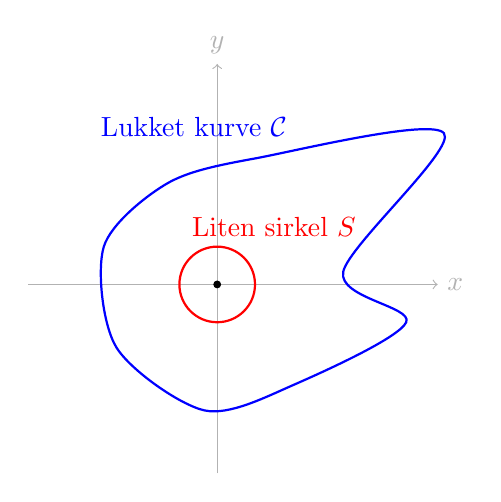
\begin{tikzpicture}[scale=0.8]
  %
  % Axes
  \draw[->, gray!60] (-3,0) -- (3.5,0) node[right] {$x$};
  \draw[->, gray!60] (0,-3) -- (0,3.5) node[above] {$y$};
  %
  % Smooth closed (simple) curve around origin with multiple arrow markers
  \draw[thick, blue]
    plot[smooth cycle] coordinates {
      (2,0.2) (3.6,2.4) (0.6,2) (-0.8,1.6) (-1.8,0.6)
      (-1.6,-1) (-0.2,-2) (1.2,-1.6) (3,-0.6)
    };
  % Small circular path around the origin (inside the closed curve)
  \draw[thick, red] (0,0) circle[radius=0.6];
  % Origin marker
  \filldraw (0,0) circle (1.5pt);
  % Labels
  \node[blue,right] at (-2,2.5) {Lukket kurve $\mathcal{C}$};
  \node[red,above] at (0.9,0.6) {Liten sirkel $S$};
\end{tikzpicture}
\end{minipage}
\end{eks}

%
\subsection{Anvendelse: Arealberegning og Green's teorem}
Husk at arealet av et område \( D \) kan beregnes ved hjelp av følgende dobbeltintegral:
\[
\text{Areal} = \iint_D dA
\]
La oss nå tenke på dette dobbeltintegralet som resultatet av Greens teorem. Med andre ord, anta at:
\[
\frac{\partial Q}{\partial x} - \frac{\partial P}{\partial y} = 1
\]
og se om vi kan finne funksjoner \( P \) og \( Q \) som tilfredsstiller dette.
Det finnes mange funksjonspar som oppfyller dette krav. For eksempel
\[
P = 0,\quad Q = x; \qquad 
P = -y,\quad Q = 0;
\qquad 
P = -\frac{y}{2},\quad Q = \frac{x}{2}
\]
Dersom vi bruker Greens teorem «baklengs», ser vi at arealet av området \( D \) også kan beregnes ved å evaluere ett av følgende linjeintegraler:
\[
A = \oint_C \begin{bmatrix} x\\ 0\end{bmatrix} \cdot \, d\mathbf{r} = -\oint_C\begin{bmatrix} 0\\ y\end{bmatrix} \cdot \, d\mathbf{r} = \frac{1}{2} \oint_C \begin{bmatrix} x\\ -y\end{bmatrix} \cdot \, d\mathbf{r}
\]
hvor \( C \) er randen til området \( D \).
\begin{eks}{Areal til en disk}
La $D$ være en disk med radius $r$. I så tilfelel er randkurven $C$ gitt med parametrisering
\[x=a\cos (t) \qquad y= a \sin(t), \quad 0\leq t \leq 2\pi \]
Vi bruker den tredje integral og finner
\begin{align*}
\text{Areal} = \frac{1}{2}\oint_C\begin{bmatrix} x\\-y\end{bmatrix} \cdot \, d\mathbf{r} = \frac{a^2}{2}\left(\int_0^{2\pi} \cos (t) (\cos(t)) dt - \sin(t) (-\sin(t)) \, dt \right) = \pi a^2
\end{align*}
\end{eks}

%
%
%
\section{Fluksintegraler i 3D}\label{sect:fluks3d}

\paragraph{Orienterbarhet av flater. }For linjeintegraler var det nødvendig å snakke om orientering av kurver når vi introduserte fluksintegraler i 2D. Det samme gjelder for flater og vi introduserer nå ideen om en \emph{orientert flate}.

La oss begynne med en flate som har to sider\footnote{husk at Möbiusbåndet, \url{https://no.wikipedia.org/wiki/Möbius-bånd} er en flate som bare har én side!}  og som har et tangentplan i hvert punkt (bortsett fra muligens langs randen). 

\begin{minipage}{6cm}
Ved å gjøre denne antakelsen, innebærer det at hvert punkt på flaten vil ha to normalvektorer, 
\[
\vect{n}_1 \quad \text{og} \quad \vect{n}_2 = -\vect{n}_1.
\]
Enhver orienterbar flate vil derfor ha to sett med normalvektorer. Det settet vi velger, vil gi flaten en orientering. 

Merk følgende definisjon.
\end{minipage}
\begin{minipage}{8cm}
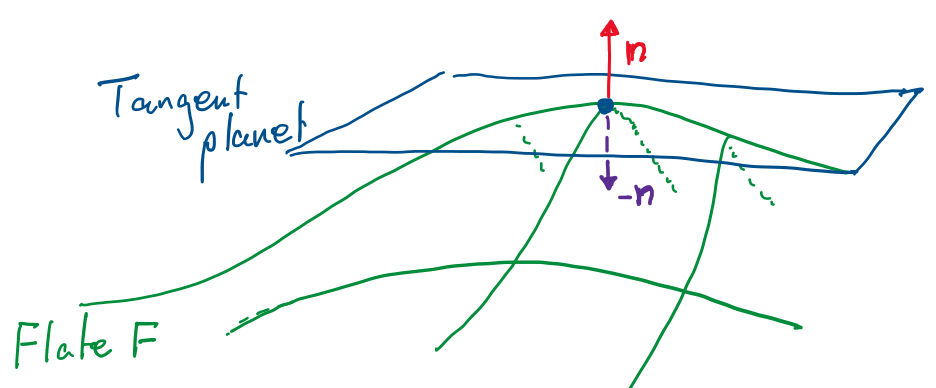
\includegraphics[width=8cm]{Fig/Flate orientering.png}
\end{minipage}

\begin{defn}{Lukket flate}
En flate $S$ er lukket dersom den utgjør randen til et volum $E$.
\end{defn}
%
Et godt eksempel på en lukket flate er overflaten til en kule eller en boks i 3D.

\begin{oppsum}{Standard orientering: Positiv orientering}
Vi sier at den lukkede flaten $S$ som er randen til $E$ har \emph{positiv orientering} dersom vi velger enhetsnormalvektorene $\hat{\vect{n}}$ til overflaten slik at de peker \emph{ut} fra området $E$, mens \emph{negativ orientering} vil si at normalvektorene peker \emph{inn} i området $E$.

Merk at denne konvensjonen kun brukes for lukkede flater.
\end{oppsum}

Vi starter med å anta at vi har et vektorfelt:
\[
\vect{F}(x, y, z) = P(x, y, z)\, \vect{i} + Q(x, y, z)\, \vect{j} + R(x, y, z)\, \vect{k}
\]
og en orientert flate \( S \) med enhetsnormalvektor \( \hat{\vect{n}}\).

\begin{defn}
\emph{Fluksintegral} av \( \vect{F} \) over \( S \) som:
\[
\iint_S \vect{F} \cdot d\vect{S} := \iint_S \vect{F} \cdot \hat{\vect{n}}\, dS
\]
Husk at $\vect{F}\cdot \hat{\vect{n}}$ tar verdier i $\R$, integralet på høyre er dermed en vanlig flateintegral (se \Cref{defn:flateintegral}).
\end{defn}

\textbf{Fysisk tolkning av fluksintegral} Fluksintegralet over en orientert flate $S, \hat{\vect{n}}$ representerer mengden av feltet som "flyter gjennom" flaten i retning av $\vect{n}$. Dette kalles også \emph{fluks} gjennom flaten.
\[
\text{Fluks} = \iint_S \vect{F} \cdot \hat{\vect{n}}\, dS \qquad \text{hvor: }
\]
\begin{itemize}
\item Positivt bidrag oppstår når \( \vect{F} \) peker i samme retning som normalvektoren $\hat{\vect{n}}$,
\item Negativt bidrag oppstår når \( \vect{F} \) peker motsatt vei.
\end{itemize}
Orientering er dermed valg av retningen på flyten vi fastsetter. 
%
\begin{rem}{Orientering og fluksintegral}
Fluksintegral (som i 2D) er avhengig av valg av en orientering. Når vi definerer integralet må vi angi hvordan vi ønsker å orientere flaten. Merk at orientering endrer bare fortegn ettersom de to enhetsnormalvektorene er relatert ved $\hat{\vect{n}}_1=-\hat{\vect{n}}_2$ og $\hat{\vect{n}}_2$ . Dermed har vi 
\[\iint_S \vect{F} \cdot \hat{\vect{n}}_2 dS = -\iint_S \vect{F} \cdot \hat{\vect{n}}_1 dS \]
\end{rem}

%
\subsection*{Formel for enhetsnormalvektoren.} Vi skal nå fremstille formler for enhetsnormalvektorer. 
Hvis flaten er lukket må vi passe på at vektorer vi konstruerer er valgt med riktig fortegn for å få positiv orientering av flaten. 
Vi har to måter å gjøre dette på, avhengig av hvordan flaten er gitt.

\begin{oppsum}{\emph{Case 1:} Flaten er en graf} Anta at flaten er gitt ved $z = g(x, y)$. I dette tilfellet definerer vi en ny funksjon
\[
f(x, y, z) = z - g(x, y).
\]
I forhold til denne nye funksjonen er flaten gitt ved ligningen $f(x, y, z) = 0$. Husk at gradienten $\nabla f$ vil være ortogonal (eller normal) på flaten som er gitt av $f(x, y, z) = 0$. Dette gir oss en normalvektor til flaten. Hvis vektoren ikke er en enhetsvektor deler vi på lengden. I vårt tilfelle er dette:
\[
\hat{\vect{n}} = \frac{\nabla f}{\|\nabla f\|} = \frac{-g_x \vect{i} - g_y \vect{j} + \vect{k}}{\sqrt{(g_x)^2 + (g_y)^2 + 1}}.
\]

Hvis flaten er gitt eksplisitt som \( z = g(x, y) \), og den har en oppoverrettet orientering (dvs. normalvektor peker i positiv \( z \)-retning), så er fluksintegralet av $\vect{F}=P\vect{i}+Q\vect{j}+R\vect{k}$:
\[
\iint_S \vect{F}\cdot d\vect{S}=\iint_S \vect{F} \cdot \hat{\vect{n}}\, dS = \iint_D \left( -P \frac{\partial g}{\partial x} - Q \frac{\partial g}{\partial y} + R \right) \sqrt{ \left( \frac{\partial g}{\partial x} \right)^2 + \left( \frac{\partial g}{\partial y} \right)^2 + 1 }\, dx\, dy
\]
Her er \( D \) projeksjonen av flaten ned på \( xy \)-planet.
\end{oppsum}

\begin{eks}{Graf eksempel}
Vi bruker $g(x,y)=2-x^2-y^2$ over $D=[0,1] \times [-1,1]$ of $\vect{F}(x,y,z)=z\vect{i}+z\vect{j}-2z(x+y)\vect{k}$ som eksempel. Der finner vi $g_x(x,y)=-2x$ og $g_y(x,y)=-2y$ og integralet blir
\[\iint_S \vect{F} \cdot d \vect{S} = \iint_D \left(2(zx+zy)-2z(x+y)\right)\sqrt{4(x^2+y^2)+1}\, dA = 0\]
Dermed er fluksen til integralet lik $0$ og det betyr at per tidsenhet netto strøm av felt $\vect{F}$ over flaten er $0$, dvs. inn og utflytt av vesken er balansert.
\end{eks}

\begin{oppsum}{Case 2: Flaten er parametrisert}
Hvis flaten \( S \) er gitt ved en parameterisering:
\[
\vect{r}(u, v) = x(u, v)\, \vect{i} + y(u, v)\, \vect{j} + z(u, v)\, \vect{k}
\]
så er fluksintegralet:
\[
\iint_S \vect{F} \cdot\, d\vect{S} = \iint_S \vect{F} \cdot \hat{\vect{n}}\, dS = \iint_D \vect{F}(\vect{r}(u,v)) \cdot (\vect{r}_u \times \vect{r}_v)\, du\, dv
\]
Her gir kryssproduktet \( \vect{r}_u \times \vect{r}_v \) en vektor normal på flaten (ikke nødvendigvis enhetslengde), og orienteringen bestemmes av retningen til dette kryssproduktet.
\begin{minipage}{\textwidth}
\begin{rem}{Standardorientering for lukkete flater} Hvis vi ha en lukket flate og ønsker standardorientering bør man sjekke om kryssproduktet faktisk peker i riktig retning!
\end{rem}
\end{minipage}
\end{oppsum}

\begin{eks}{Parametrisert flate som ikke er en graf}\label{ex:halvkule}
Gitt \( \vect{F}(x, y, z) = x\, \vect{i} + y\, \vect{j} + z\, \vect{k} \), og \( S \) er flaten av halvkule \( x^2 + y^2 + z^2 = 1 \), \( z \geq 0 \), vi ønsker fluksintegral med hensyn til utadrettet normal.
Da bruker vi parameteriseringen av halvkulen ved hjelp av kulekoordinater:
\[
\vect{r}(u, v) = \sin u \cos v\, \vect{i} + \sin u \sin v\, \vect{j} + \cos u\, \vect{k}, \quad 0 \leq u \leq \frac{\pi}{2},\ 0 \leq v \leq 2\pi
\]
For å beregne normalvektor har vi to muligheter: 
\begin{align*}
\vect{r}_u \times \vect{r}_v &= \begin{vmatrix}
   \vect{i} & \vect{j} & \vect{k} \\
   \cos u \cos v & \cos u \sin v & - \sin u \\
   -\sin u \sin v & \sin u \cos v & 0 
\end{vmatrix} \\&= (\sin u)^2\cos v \vect{i}+(\sin u)^2\sin v \vect{j}+\sin u  \cos u \vect{k}
\end{align*}
I hvilken retning peker vektoren? Siden det  kan ikke flippe over er det nok å sjekke ved et punkt:\footnote{Det er en dårlig id\'{e} å bruke $u=0$ her. Hvorfor og hva er geometrisk betydning til det?} $\vect{r}_u \times \vect{r}_v (\pi/4,0)= 1/2(\vect{i}+2\vect{k}$, og på $\vect{r}(\pi/4,0)=\sqrt{2}/2(\vect{i}+\vect{k})$ peker det ut av halvkulen. Dermed stemmer retning. Vi evaluerer nå integralet:
\begin{align*}
&\iint_S \vect{F} \cdot d\vect{S} = \iint_D \vect{F}(\vect{r}(u,v)) \cdot (\vect{r}_u \times \vect{r}_v)\, du\, dv\\
=& \int_0^{2\pi}\int_0^{\pi/2} (\sin u)^3(\cos v)^2 + (\sin u)^3(\sin v)^2 + \sin (u)(\cos v)^2 \, du dv \\ =& \int_0^{2\pi}\int_0^{\pi/2} \frac{3\sin u - \sin (3u)}{4} + \sin (u)(\cos v)^2 \, du dv \\ =& \int_0^{2\pi}\left. \frac{-9\cos (u) +\cos (u)}{12}-\cos (u)(\cos v)^2\right|_{u=0}^{u=\pi/2} dv = \frac{4}{3}\pi + \int_0^{2\pi}
 (\cos v)^2 dv\\
 =& \frac{4}{3}\pi + \int_0^{2\pi} \frac{1-\cos (2v)}{2} dv =  \frac{4}{3}\pi+ \left. \frac{4v-\sin (2v)}{8}\right|_{0}^{2\pi} = \frac{4}{3}\pi+\pi = \frac{7}{3}\pi \end{align*}
\end{eks}
%
Vi avslutter med et eksempel av en lukket flate som er sammensatt av to flater som - hver for seg - er enkelt å parametrisere.
\begin{eks}{Sammensatt flate}
La $\hat{S}$ være flaten som begrenser $E=\{(x,y,z) \colon x^2+y^2+z^2\leq 1, z \geq 0\}$. 
Da er $\hat{S}$ lukket og sammensatt av halvkulen $S$ fra \Cref{ex:halvkule} og enhetsdisken $D$ i $xy$-planet. 
Vi ønsker å beregne fluksintegral for $\vect{F}(x,y,z)=x\vect{i}+y\vect{j}+z\vect{k}$
med positiv orientering av $\hat{S}$. 
For dette bruker vi 
\begin{align*}
\iint_{\hat{S}} \vect{F} \cdot d \vect{S} = \iint_S \vect{F} \cdot d \vect{S} + \iint_D \vect{F} \cdot d \vect{S} = \frac{7}{3} \pi + \iint_D \vect{F} \cdot d \vect{S} 
\end{align*}
Siden vi allerede har beregnet det første integralet i siste eksempel. 
Nå parametriserer vi $D$ som
\[x= r \sin \theta , \quad y = r \cos \theta, \quad z =0, \qquad 0 \leq r \leq 1, 0\leq \theta \leq 2 \pi\]
En enkelt regning (kryssprodukt!) viser at $\vect{n}(r,\theta) = -r \vect{k}$.
\footnote{normalvektoren forsvinner her faktisk i origo. Det uttrykker singulariteten av polarkoordinater i origo. Siden integraler bryr seg ikke om enkle punkter kan vi ignorere det!}, og dermed får vi \[\iint_D \vect{F}(r\cos \theta, r \sin \theta,0) \cdot \vect{n}(r,\theta) dr d\theta = 0   \]
Oppsummert: $\iint_{\hat{S}} \vect{F} \cdot d \vect{S} = \iint_S \vect{F} \cdot d \vect{S} = \frac{7}{3}\pi$
\end{eks}

%
%
%
\section{Divergenssetningen (Gauss' teorem)}\label{sect:gauss}

I denne seksjonen skal vi knytte sammen flateintegraler og trippelintegraler. 
Dette gjør vi ved hjelp av \textbf{divergenssetningen}. 
Den følger det generelle mønsteret til de andre integralteoremene vi har sett.  
Dersom vi tenker på divergens som en slags derivasjon, sier divergenssetningen at et trippelintegral av den deriverte 
$\nabla \cdot \mathbf{F}$ over et volum henger sammen med et fluksintegral av \(\mathbf{F}\) over randflaten til volumet. 

\begin{thm}[Divergenssetningen (Gauss' teorem)] \label{thm:divergens}
La \( V \) være et enkelt, lukket tredimensjonalt område og \( S \) være randflaten\footnote{Enkelt og lukket betyr her at volum ikke har noen hull. 
Videre antar vi at randflaten til området består av stykkevis glatte randflater, dvs.\ det er mulig å beregne en normalvektor} til \( V \), med normalvektor $\vect{n}$ som peker ut av volumet. 
La \( \vect{F} \) være et vektorfelt der komponentene har kontinuerlige førsteordens partielllderiverte. 
Da gjelder:
\[
\iint_S \vect{F} \cdot d\vect{S} = \iiint_V \mathrm{div} \, \vect{F} \, dV
\]
\end{thm}

\begin{figure}[htpb] \centering
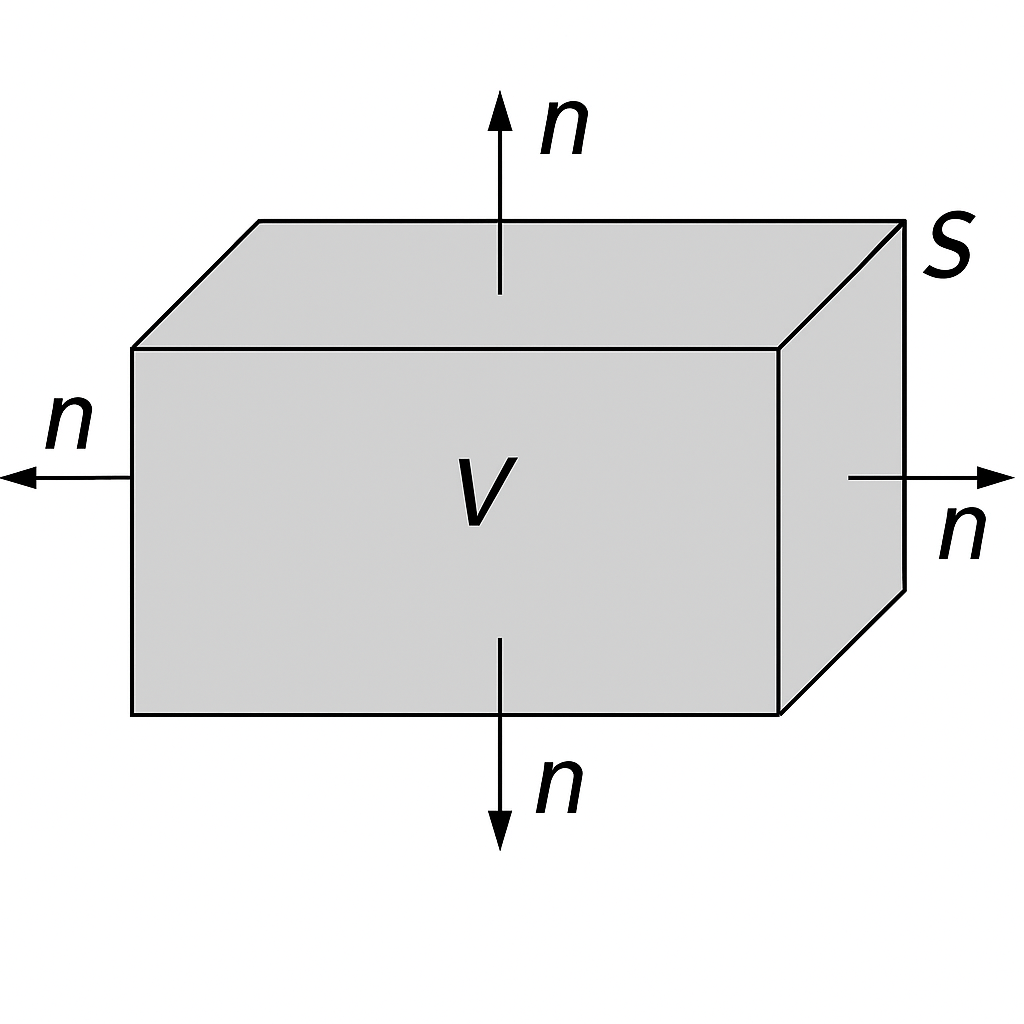
\includegraphics[width=10cm]{Fig/DivBoks.png}
\caption{Tredimensjonalt volum $V$ med randflate $S$ og normalvektor $\vect{n}$ som peker ut. Kilde: \href{https://en.wikipedia.org/wiki/Divergence_theorem}{Wikipedia}, \href{https://creativecommons.org/licenses/by-sa/3.0/}{CC BY-SA 3.0}.}
\end{figure}

\begin{eks}{Fluks gjennom en kube}
La $\vect{F}(x,y,z)= \frac{-y}{z}\vect{i}+\frac{x}{z}\vect{j}$ være strømningsfelt til en væske og $C$ en kube gitt ved \[1 \leq x \leq 4, \quad 2\leq y \leq 5, \quad -5 \leq z \leq -2.\]
Beregn fluksen gjennom overflaten $\partial C$ til $C$.

Før vi beregner $\iint_{\partial C} \vect{F} \cdot d \vect{S}$, skal vi diskutere hva verdien av integralet bør være. 
Vektorfeltet er rotasjonelt av natur, og for en sirkel parallell med \(xy\)-planet med sentrum på \(z\)-aksen, 
har vektorene langs denne sirkelen samme lengde. 
Dette viser at strømmen inn og ut av kuben er den samme. 
Strømmen som går inn i kuben kansellerer strømmen som går ut, og derfor bør netto fluks gjennom kuben være null.

For å bekrefte denne intuisjonen må vi beregne fluksintegralet. 
Å beregne fluksen direkte krever at vi deler integralet opp i seks separate fluksintegraler - 
ett for hver sideflate av kuben. 
Vi må også finne tangentvektorer og beregne kryssproduktet deres.  
Men ved å bruke divergensteoremet går denne beregningen mye raskere:
\[
\iint_{\partial C} \mathbf{F} \cdot d\mathbf{S} 
= \iiint_{C} (\nabla \cdot \mathbf{F}) \, dV = \iiint_{C} 0 \, dV=0
\]
Ettersom \(\nabla \cdot \mathbf{F} = 0\), får vi at fluksen er null, slik vi forventet.
\end{eks}

\begin{eks}{Regneeksempel for sammensatt flate}
Bruk divergenssetningen til å beregne  
\[
\iint_S \vect{F} \cdot d\vect{S} \text{ hvor } \vect{F} = xy\,\vect{i} - \frac{1}{2} y^2\,\vect{j} + z\,\vect{k}
\]  
og flaten \( S \) består av tre deler:
\begin{itemize}
  \item Toppen: \( z = 4 - 3x^2 - 3y^2 \), for \( 1 \leq z \leq 4 \)
  \item Sidene: \( x^2 + y^2 = 1 \), for \( 0 \leq z \leq 1 \)
  \item Bunnen: \( z = 0 \)
\end{itemize}
Området \( E \) er omsluttet av disse flatene. Vi bruker sylinderkoordinater:
\[
0 \leq z \leq 4 - 3r^2,\quad 0 \leq r \leq 1,\quad 0 \leq \theta \leq 2\pi
\]
Divergensen er:
\[
\text{div} \, \vect{F} = \frac{\partial}{\partial x}(xy) + \frac{\partial}{\partial y}\left(-\frac{1}{2}y^2\right) + \frac{\partial}{\partial z}(z) = y - y + 1 = 1
\]
Da blir integralet:
\begin{align*}
\iint_S \vect{F} \cdot d\vect{S} &= \iiint_E 1 \, dV = \int_0^{2\pi} \int_0^1 \int_0^{4 - 3r^2} r \, dz \, dr \, d\theta \\
&= \int_0^{2\pi} \int_0^1 r(4 - 3r^2) \, dr \, d\theta = \int_0^{2\pi} \left[2r^2 - \frac{3}{4}r^4\right]_0^1 d\theta = \int_0^{2\pi} \frac{5}{4} \, d\theta = \frac{5}{2} \pi
\end{align*}
\end{eks}

\paragraph{Spesialversjon av Gauss' lov ved konservativt vektorfelt}
La oss se på en spesiell situasjon hvor $S \subseteq \R^3$ er en orientert lukket flate rundt et volum $V$ og vi ser på en spesiell type vektorfelt 
\[\vect{F}(x,y,z):= \phi(x,y,z)\vect{i}\]
Husk (se \Cref{app:diffop_ident}) at det finnes en produktregel for divergens:
\[\text{div} (\phi \vect{i})=\phi \underbrace{\text{div} (\vect{i})}_{=0} + \text{grad } \varphi \cdot \vect{i} = \text{grad } \varphi \cdot \vect{i}.\] 
Vi setter dette inn i  divergensteoremet \Cref{thm:divergens}:
\begin{align}\label{Grad_gauss}
\iiint_V \text{grad} (\phi) \cdot \vect{i} dV = \iiint_V  \text{div} (\phi\vect{i})\,dV= \iint_S (\phi \vect{i}) \cdot d\vect{S} = \iint_S \phi \vect{i} \cdot \hat{\vect{n}}\, dS 
\end{align}
Husk at for en vilkårlig vektor $x\vect{i}+y\vect{j}+z\vect{k}$ prikkprodukt med $\vect{i}$ gir første komponent $x$. 
Så \eqref{Grad_gauss} sier at volumintegralet over første komponent til $\text{grad} \phi$ er lik flateintegral til første komponent til $\phi \hat{\vect{n}}$. 
Istedet av $\vect{i}$ kunne vi ha regnet med $\vect{j}$ eller $ \vect{k}$. 
Dette gir oss:

\begin{prop}[Gradientversjon for Gauss` teorem]\label{prop:gauss_grad}
    For $S=\partial V$ en flate som oppfyller forutsetninger til Gauss' teorem og en kontinuerlig deriverbar funksjon $\phi$ gjelder
    \[\iiint_V \mathrm{grad }\, \phi \, dV = \iint_S \phi \hat{\vect{n}}\, dS.\]
    Hvor integralene til vektorer er tatt komponentvis.
\end{prop}

%
\subsection{Anvendelse: Maxwell's ligninger}
På 1800-tallet skrev Maxwell ned likningene som beskriver elektrisitet og magnetisme. 
For å formulere likningene må vi utvide begrepet vektorfelt litt:

\begin{defn}{Tidsavhengig vektorfelt}
    En funksjon\footnote{Eller mer generelt en funksjon som er definert på en åpen mengde i $\R^n \times \R$ med verdier i $\R^n$.} $E \colon \R^n \times \R \rightarrow \R^n$ kaller vi \emph{tidsavhengig vektorfelt}.
\end{defn}
\textbf{Obs}: Hvis $E$ er et tidsavhengig vektorfelt, så er for hver $t \in \R$ $E(\cdot, t) \colon \R^n  \rightarrow \R^n$ et vanlig vektorfelt. 
Det forklarer hvorfor vi kaller de \emph{tidsavhengige} vektorfelt.

På differensialform (hvor vi bruker $\nabla$ operator som er populær i fysikk) ser Maxwell sine likningene slik ut:
\begin{oppsum}{Maxwell's likninger}
\begin{align}\label{max:divEB}
\nabla \cdot \vect{E} = \frac{\rho}{\varepsilon}  &\qquad \nabla \cdot \vect{B} = 0 \\
\nabla \times \vect{E} = -\frac{\partial \vect{B}}{\partial t} & \qquad \nabla \times \vect{B} = \mu \left( \vect{J} + \varepsilon \frac{\partial \vect{E}}{\partial t} \right) \label{max:PDE}
\end{align}
Her er \( \vect{E}(x, t) \) og \( \vect{B}(x, t) \) vektorfelter som representerer henholdsvis elektrisk og magnetisk feltstyrke, mens \( \rho(x, t) \) og \( \vect{J}(x, t) \) er henholdsvis ladningstetthet (C/m³) og strømtetthet (A/m²). 

Videre er \( \varepsilon \) den elektriske permittiviteten (hvor lett et stoff lar seg polarisere), og \( \mu \) er den magnetiske permeabiliteten (et materiales evne til å la seg magnetisere). Vi antar her at både \( \varepsilon \) og \( \mu \) er skalare konstanter\footnote{Men generelt er de tensorielle størrelser.}. Vakuumpermittiviteten \( \varepsilon_0 \) og vakuumpermeabiliteten \( \mu_0 \) oppfyller relasjonen:
\[
c_0 = \frac{1}{\sqrt{\mu_0 \varepsilon_0}} = 2.99792458 \times 10^8\ \text{m/s},
\]
som også er lyshastigheten i vakuum. 
\end{oppsum}

\begin{rem}{}
Husk notasjon \eqref{max:divEB} er ligninger for divergens mens \eqref{max:PDE} er ligninger for rotasjon.

Dessuten er \eqref{max:PDE} en ligning som involverer både deriverte i rom retninger $x,y,z$ og med hensyn til tid $t$. Detter er et første eksempel av en partiell differensialligning (PDE) vi skal se nærmere på i \Cref{sect:PDE}
\end{rem}
\begin{eks}{Elektrisk felt rundt statisk ladningsfordeling}
La oss finne den elektriske feltstyrken \( \vect{E}(\vect{r}) \) utenfor en sfærisk-symmetrisk, statisk ladningsfordeling 
\[
Q = \iiint \rho(\vect{r})\, dV
\]
Vi skal vise at:
\[
\vect{E}(\vect{r}) = \frac{1}{4 \pi \varepsilon_0} \frac{Q}{r^2} \hat{r}
\]
der \( r = \sqrt{x^2 + y^2 + z^2} \) og \( \hat{r} = \vect{r}/r \).
Fra Maxwells likninger, \eqref{max:divEB} får vi:
\[
\iiint \nabla \cdot \vect{E}\, dV = Q
\]
Ved Gauss’ lov \Cref{thm:divergens}:\Ben{I assume $E$ is a constant only depending on the radius (which makes sense physically to assume that this is what it needs to be, we should introduce it though beforehand){\color{blue} Ben: Yes, the symmetry of the problem would require that. I will include a better discussion}}
\begin{align*}
\iiint \nabla \cdot \vect{E}\, dV = \iint \vect{E} \cdot d\vect{S} = E(r) \hat{r} \cdot \hat{r} \iint dS = 4\pi r^2 E(r)
\\
\Rightarrow \vect{E}(\vect{r}) = \frac{1}{4 \pi \varepsilon_0} \frac{Q}{r^2} \hat{r}
\end{align*}
\end{eks}

%
\subsection{Anvendelse: Arkimedes' lov}
Arkimedes lov er et velkjent resultat om oppdrift fra antikken. Den ble formulert av \href{https://no.wikipedia.org/wiki/Arkimedes}{Arkimedes} fra Syrakus i Italia. Du kan lære mer om Arkimedes lov \href{https://www.youtube.com/watch?v=euvIlejovCA&list=PLBSPq-MdQqruVxoeYU6tAZ9t-kDUXXhoE&index=6}{her}. Loven går som følger. Anta at et legeme plasseres i ei væske. Da gjelder:

\begin{oppsum}{Arkimedes' lov}
Oppdriftskraften $\vect{F}_\textrm{oppdrift}$ på et legeme nedsenket i en væske er like stor som tyngden $\vect{G}_\textrm{fortrengt}$ av væsken som legemet fortrenger. I og med at oppdriftskraften peker oppover, mens tyngdekraften peker nedover så har vi 
\begin{equation}
    \label{arkimedes}
    \vect{F}_\textrm{oppdrift}=-\vect{G}_\textrm{fortrengt}.
\end{equation}
\end{oppsum}
I det følgende eksemplet skal vi bruke Gauss' lov for å beregne oppdriftskraften på et legeme nedsenket i vann. For å gjøre det har vi også behov for likningen som angir trykket i ei væske som funksjon av høyden. Dette kalles loven om hydrostatisk trykk. Den utledes \href{https://www.youtube.com/watch?v=RpJu9hDTsGU&list=PLBSPq-MdQqruVxoeYU6tAZ9t-kDUXXhoE&index=5}{her}, og resultatet går som følger. Trykket (altså kraften per areal) i ei væske på jordas overflate, er gitt ved

\begin{equation}
    p(z)=\rho\textrm{g}z+p_0
\end{equation}
hvor $z$ er dybden under væskeoverflaten og $p_0$ er overflatetrykket. Merk at nå  
\begin{equation}
\label{gradp}
    \nabla p = \rho g\vect{k} = -\rho\vect{g},
\end{equation}
hvor $\vect{g}=-\textrm{g}\vect{k}$, hvor $\textrm{g}\approx 9.81\textrm{m}/\textrm{s}^2$ er gravitasjonens akselerasjon ved jordoverflaten. Sammenhengen mellom trykk og kraft; $p=dF/dS$ gir oss dessuten kraften som følge av trykkforskjell (som i Gradientversjonen av Gauss teorem er integralene tenkt komponentvis dersom vi integrerer en vektorverdi funksjon);
\begin{align}
\label{trykkraft}
   \vect{dF}= p d\vect{S} \quad\Rightarrow \quad \vect{F}=\iint_S p\hat{\vect{n}} \,dS,
\end{align}
hvor $S$ er overflaten til legemet det øves trykkrefter på. Her er det altså viktig å merke seg at trykkreftene står normalt på overflaten, og at de er de samme i samme høyde. For et legeme nedsenket i vann vil netto kraft derfor kunne være som følge av trykk i vertikal retning. Altså reduserer \eqref{trykkraft} til
\begin{align}
\label{trykkraft2}
\vect{F}_\textrm{oppdrift}=\iint_S p\vect{k}\, dS.
\end{align}

\begin{eks}{Arkimedes' lov}
La $S$ være overflaten på en lukket flate som oppfyller antagelsene i Gauss' \Cref{thm:divergens}, slik som en badeball. Anta videre at badeballen er nedsenket i vann. Med andre ord utgjør volumet til badeballen, $V \subseteq \R^3$ et volum omgitt av ei væske. Massen til det fortrengte vannet kaller vi $m_\textrm{fortrengt}$. La $\rho$ være tettheten til vannet. Da har vi følgende uttrykk for kreftene (integraler forstås komponentvis):
\begin{align}
\label{fortrengt}
\vect{G}_\textrm{fortrengt}&=m_\textrm{fortrengt}\vect{g}=\iiint_V\rho \vect{g} dV\overset{\eqref{gradp}}{=}-\iiint \nabla p\, dV \stackrel{\Cref{prop:gauss_grad}}{=}-\iint_{S} p \hat{\vect{n}}\, dS\notag\\
&=-\iint_{S} p\vect{k} \,dS\overset{\eqref{trykkraft2}}{=}-\vect{F}_\textrm{oppdrift}.\notag
\end{align}
\end{eks}
Sjekk \cite{Lima} for mer informasjon om Arkimedes' lov og hvordan forskjellige varianter kan begrunnes ved hjelp av Gauss teorem.

%
%
%
\section{Stokes' teorem}\label{sect:stokes}

Vi skal se på Stokes' teorem som er en høyere-dimensjonal versjon av Green`s teorem. 
I Green`s teorem relaterte vi et linjeintegral til et dobbeltintegral over et område. 
I dette avsnittet skal vi relatere et linjeintegral til et flateintegral. 
Før vi presenterer teoremet, må vi først definere kurven som brukes i linjeintegralet.
La oss starte med følgende orientert flate (hvor $\vect{n}$ er valgt normalvektor).

\begin{minipage}{7cm}
Rundt kanten av denne flaten har vi en kurve $C$. Denne kurven kalles randkurven. Orienteringen til flaten $S$ induserer den positive orienteringen til $C$. For å finne den positive orienteringen av $C$, tenk deg at du går langs kurven. Hvis hodet ditt peker i samme retning som enhetsnormalene og flaten er på din venstre side, så går du i positiv retning langs $C$.
\end{minipage}
\begin{minipage}{7cm}
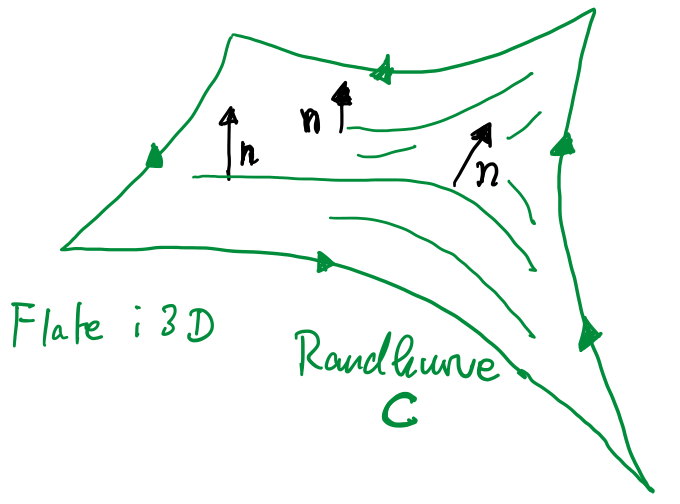
\includegraphics[width=7cm]{Fig/stokes_ orientering.png}
\end{minipage}

\begin{oppsum}{Standard orientering for randkurver av flater}
For en orientert flate $S,\vect{n}$ med randkurve $C$ skal vi i alt som følger velge en parametrisering til $C$ som samsvarer positiv orientering av $C$ som randkurve av $S$. 
\end{oppsum}

\begin{thm}[Stokes' Teorem]\label{thm:stokes}
La $S$ være en orientert glatt flate begrenset av en enkel, lukket og glatt randkurve $C$ med positiv orientering. La også $\vect{F}$ være et vektorfelt. Da gjelder:
\[
\oint_C \vect{F} \cdot d\vect{r} =\iint_S \operatorname{curl} \vect{F} \cdot d\vect{S} = \iint_S \nabla \times \vect{F} \cdot d\vect{S}
\]
\end{thm}
I Stokes teorem kan flaten $S$ faktisk være hvilken som helst flate, så lenge randkurven er gitt av $C$. Dette kan utnyttes for å forenkle flateintegralet.


\begin{eks}{}
Bruk Stokes’ teorem til å evaluere
\[
\oint_C \vect{F} \cdot d\vect{r} \quad \text{ der } \vect{F} = z^2 \vect{i} + 42y \vect{j} + x \vect{k}
\]
og $C$ er trekanten med hjørner $(1, 0, 0)$, $(0, 1, 0)$ og $(0, 0, 1)$, orientert mot klokken.

Vi trenger curl av vektorfeltet:
\[
\nabla \times \vect{F} = \begin{vmatrix}
\vect{i} & \vect{j} & \vect{k} \\
\frac{\partial}{\partial x} & \frac{\partial}{\partial y} & \frac{\partial}{\partial z} \\
z^2 & 42y & x
\end{vmatrix}
= (2z - 1)\vect{j}
\]
Bruk planet $x + y + z = 1 \Rightarrow z = 1 - x - y$ som flate med oppover-orientering. Dermed er 
\[
f(x, y, z) = z - (1 - x - y) = z - 1 + x + y
\Rightarrow \nabla f = \vect{i} + \vect{j} + \vect{k}
\]
Området $D$ i $xy$-planet er trekanten med hjørner $(0,0)$, $(1,0)$ og $(0,1)$.
Integralet blir:
\begin{align*}
\oint_C \vect{F} \cdot d\vect{r}
&= \iint_D (2z - 1) \vect{j} \cdot \frac{\nabla f}{\|\nabla f\|} dA
= \int_0^1 \int_0^{-x + 1} (1 - 2x - 2y) \, dy \, dx\\
&= \int_0^1 \left[ y - 2xy - y^2 \right]_0^{-x+1} dx
= \int_0^1 (x^2 - x) \, dx
= \left[\frac{1}{3}x^3 - \frac{1}{2}x^2 \right]_0^1
= -\frac{1}{6}
\end{align*}
\end{eks}

Vektoranalyse spiller en sentral rolle i teorien om elektromagnetisme. Det neste eksemplet viser hvordan Stokes’ teorem anvendes.

\begin{eks}{Faraday's lov}
La \( \mathbf{E} \) og \( \mathbf{H} \) være tidsavhengige elektriske og magnetiske felt i rommet. La \( S \) være en flate med rand \( C \). Vi definerer
\[
\int_C \mathbf{E} \cdot d\mathbf{r} = \text{spenningen rundt } C,
\qquad
\iint_S \vect{H} \cdot d\vect{S} = \text{magnetisk fluks gjennom } S.
\]
\begin{minipage}{8cm}
Bildet til høyre illustrerer den standardsituasjonen av en magnet og en flate rundt magneten hvor vi kan anvende   
\begin{oppsum}{Faradays lov} Spenningen rundt \( C \) er lik den negative tidsderiverte av den magnetiske fluksen gjennom \( S \). 
\end{oppsum}
\end{minipage}
\begin{minipage}{6cm}
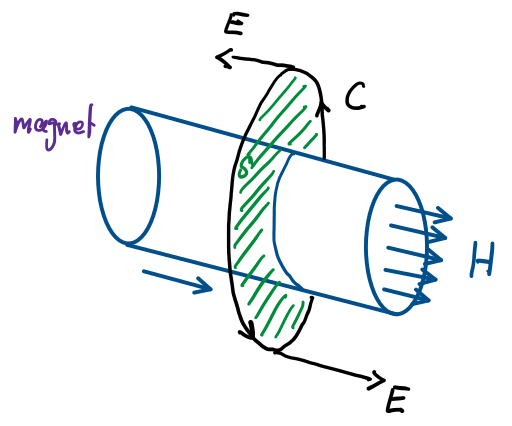
\includegraphics[width=6cm]{Fig/Faraday.png}
\end{minipage}

Vi skal vise hvordan Faradays lov følger fra en av Maxwells ligninger, \eqref{max:PDE}:
\[
\nabla \times \mathbf{E} = -\frac{\partial \mathbf{H}}{\partial t}.
\]
Anta at \( -\frac{\partial \mathbf{H}}{\partial t} = \nabla \times \mathbf{E} \). Ved bruk av Stokes’ teorem \Cref{thm:stokes} får vi
\[
\int_C \mathbf{E} \cdot d\vect{r} = \iint_S (\nabla \times \mathbf{E}) \cdot d\mathbf{S}.
\]
Vi anta at det er lov å trekke \( \frac{\partial}{\partial t} \) inn i integralet, for å få
\[
- \frac{\partial}{\partial t} \iint_S \mathbf{H} \cdot d\mathbf{S}
= \iint_S -\frac{\partial \mathbf{H}}{\partial t} \cdot d\mathbf{S}
= \iint_S (\nabla \times \mathbf{E}) \cdot d\mathbf{S}
= \int_C \mathbf{E} \cdot d\mathbf{S}.
\]
Dermed
\[
\int_C \mathbf{E} \cdot d\mathbf{s} = - \frac{\partial}{\partial t} \iint_S \mathbf{H} \cdot d\mathbf{S}. \qquad \text{(Faradays lov)}
\]
\end{eks}

En kanksje litt morsommere anvendelse av Stokes' teorem finnes i \cite[s. 249-250]{MaT88}.

%
\subsection*{Fallende katter og Stokes’ teorem}
Har du noen gang lurt på hvordan en fallende katt klarer å rette seg opp? 
Når den slippes fra hvile med beina over hodet, klarer katten å utføre en 180-graders reorientering og lande trygt på beina. 
Dette velkjente fenomenet har fascinert folk i mange år – spesielt i byer som New York, hvor katter er kjent for å ha overlevd fall fra 8 til 30 etasjer!

Det har vært mange feilaktige forklaringer på hvordan katter klarer å rette seg opp, inkludert idéen om at det har å gjøre med hvordan katten snurrer på halen. 
Dette kan ikke stemme, ettersom manx-katter, som ikke har hale, også kan utføre denne bragden!

Hvis man observerer en fallende katt\footnote{Perfekt tidspunkt for en kattevideo på \href{https://www.youtube.com/watch?v=NCRSafiD4BY}{Youtube}.} ser man at det 
retter seg opp ved å
vri på kroppsdeler.
Ved første øyekast gir det en tilsynelatende motsetning; siden katten slippes fra en hvilende posisjon, har den null dreiemoment i starten av fallet, og ifølge en grunnleggende fysikklov kalt bevaring av dreiemoment, må katten ha null dreiemoment gjennom hele fallet. Utrolig nok har katten klart å endre sin vinkelposisjon samtidig som den hele tiden har hatt null dreiemoment! \Ben{[NOTE TO SELF [BEN] Husk å skrive om litt]}

Den nøyaktige prosessen som gjør dette mulig er subtil;  Interessant nok er det Stokes’ teorem som er nøkkelen til å forstå denne typen fenomener, se \cite{Bat_cat}.


\FloatBarrier